%
% File nodalida2025.tex
%
% Contact: Sara Stymne
% Email:  sara.stymne@lingfil.uu.se
%
% Based on the instruction file for NoDaLiDa 2023 by Mark Fishel which in turn were
% Based on the instruction file for NoDaLiDa 2021 by Lilja Øvrelid which in turn were
% Based on the instruction file for NoDaLiDa 2019 by Barbara Plank and Mareike Hartmann which in turn were based on the instruction files from NoDaLiDa 2017 and 2015 by
% Beata Megyesi (beata.megyesi@lingfil.uu.se) and EACL 2014
% which in turn was based on the instruction files for previous
% ACL and EACL conferences. The BibTeX file is based on NAACL 2019
% style files, which in turn are based on style files for ACL 2018 and NAACL 2018, which were
% Based on the style files for ACL-2015, with some improvements
% taken from the NAACL-2016 style
% Based on the style files for ACL-2014, which were, in turn,
% based on ACL-2013, ACL-2012, ACL-2011, ACL-2010, ACL-IJCNLP-2009,
% EACL-2009, IJCNLP-2008...
% Based on the style files for EACL 2006 by
% e.agirre@ehu.es or Sergi.Balari@uab.es
% and that of ACL 08 by Joakim Nivre and Noah Smith

\documentclass[11pt]{article}
\usepackage{nodalida2025}
\usepackage{times}
\usepackage{url}
\usepackage{graphicx}
\usepackage{caption}
\usepackage{latexsym}
\usepackage{diagbox}
\usepackage{float}
\usepackage{nicematrix}
\usepackage{multirow}
\usepackage{enumitem}
\usepackage{amsmath, amsfonts, amssymb, amsthm, mathrsfs, stmaryrd}
\usepackage{booktabs}
\usepackage{tikz}
\usepackage{multicol}
\usepackage{colortbl}
\usepackage{pgfplots}
\usepackage{pgfplotstable}
\usepackage{hyperref}
\usepackage{tikz-dependency}

\newcommand{\scsf}[1]{\textsc{\textsf{#1}}} % Descriptive Categories

\captionsetup{belowskip=0pt, aboveskip=6pt}

\pgfplotsset{compat=1.18}
\pgfplotstableset{
  /color cells/min/.initial=0,
  /color cells/max/.initial=1000,
  /color cells/textcolor/.initial=,
  %
  % Usage: 'color cells={min=<value which is mapped to lowest color>,
  %  max = <value which is mapped to largest>}
  color cells/.code={%
    \pgfqkeys{/color cells}{#1}%
    \pgfkeysalso{%
      postproc cell content/.code={%
        %
        \begingroup
        %
        % acquire the value before any number printer changed
        % it:
        \pgfkeysgetvalue{/pgfplots/table/@preprocessed cell content}\value
        \ifx\value\empty
          \endgroup
        \else
        \pgfmathfloatparsenumber{\value}%
        \pgfmathfloattofixed{\pgfmathresult}%
        \let\value=\pgfmathresult
        %
        % map that value:
        \pgfplotscolormapaccess
          [\pgfkeysvalueof{/color cells/min}:\pgfkeysvalueof{/color cells/max}]
          {\value}
          {\pgfkeysvalueof{/pgfplots/colormap name}}%
        % now, \pgfmathresult contains {<R>, <G>, <B>}
        %
        % acquire the value AFTER any preprocessor or
        % typesetter (like number printer) worked on it:
        \pgfkeysgetvalue{/pgfplots/table/@cell content}\typesetvalue
        \pgfkeysgetvalue{/color cells/textcolor}\textcolorvalue
        %
        % tex-expansion control
        % see https://tex.stackexchange.com/questions/12668/where-do-i-start-latex-programming/27589#27589
        \toks0=\expandafter{\typesetvalue}%
        \xdef\temp{%
          \noexpand\pgfkeysalso{%
            @cell content={%
              \noexpand\cellcolor[rgb]{\pgfmathresult}%
              \noexpand\definecolor{mapped color}{rgb}{\pgfmathresult}%
              \ifx\textcolorvalue\empty
              \else
                \noexpand\color{\textcolorvalue}%
              \fi
              \the\toks0 %
            }%
          }%
        }%
        \endgroup
        \temp
        \fi
      }%
    }%
  }
}
%\aclfinalcopy % Uncomment this line for the final submission

%\title{Instructions for NoDaLiDa/Baltic-HLT 2025 Proceedings}



\title{Comparative Concepts or Descriptive Categories: a UD Case study}


\author{Anonymous Author \\
 Affiliation / Address line 1 \\
 Affiliation / Address line 2 \\
 Affiliation / Address line 3 \\
 {\tt email@domain} \\\And
 Anonymouser Author \\
 Affiliation / Address line 1 \\
 Affiliation / Address line 2 \\
 Affiliation / Address line 3 \\
 {\tt email@domain} \\\And
 Anonymousest Author \\
 Affiliation / Address line 1 \\
 Affiliation / Address line 2 \\
 Affiliation / Address line 3 \\
 {\tt email@domain} \\}

% \author{Mathieu Dehouck \\ % J'ai mis nos noms dans le préordre défini par le nombre de `t` dans le prénom.
%  Affiliation / Address line 1 \\
%  Affiliation / Address line 2 \\
%  Affiliation / Address line 3 \\
%  {\tt email@domain} \\\And
%  Matthieu Pierre Boyer \\
%  Lattice\\
%  DI ENS\\
%  Paris, France\\
%  {\tt matthieu.boyer@ens.fr} \\}

\date{}

\begin{document}
\maketitle
\begin{abstract}
In this paper, we present a series of methods used to quantify the soundness of using the same names to annotate cases in different languages.
We follow the idea described by Martin Haspelmath that descriptive categories and comparative concepts are different objects and we look at the necessary simplification taken by the Universal Dependencies project.
We thus compare cases in closely related languages as belonging to commensurable descriptive categories.
Then we look at the corresponding underlying comparative concepts.
Before eventually looking at the possibility to assign cases to adpositions.
%We use our findings to derive conditions for coherent annotations as well as ways to annotate replacements of cases in case-free languages.
\end{abstract}

\section{Introduction}

\begin{quote}
    There is a fundamental distinction between language-particular categories of languages (which descriptive linguists must describe by descriptive categories of their descriptions) and comparative concepts (which comparative linguists may use to compare languages).
    {\begin{flushright}\textit{Martin Haspelmath} in \cite{Has18}\end{flushright}}
\end{quote}

Language description and language comparison are two intertwined yet distinct endeavours.
Language description is often done in a language different from the one being described (many grammars have been written in English, French, Russian, Spanish and Portuguese for example) and often uses a conventionalised descriptive meta-language associated with a given descriptive school.
Language comparison relies on the previous step of language description as it main data source but also needs a common meta-language to name the various phenomena under study.

In his paper, \newcite{Has18} warns us against the confusion of the different meta-languages (the descriptive languages used in each individual description and the common comparative meta-language).
He advocates for a careful choice of terms when describing similar categories across multiple languages, even when the similarities compel us to use the same term.
%That is, one should not use a same word to describe two different concepts in two different languages.
That is, one should avoid using a single term to describe two categories from two different languages.
Even more so, when this term is also used as a comparative concept which then further increases the risk of cross-meta-language confusion.

With all its qualities, the Universal Dependencies (UD) project \cite{UD214} puts itself exactly in this somewhat uncomfortable situation.
One of the main aims of the project is to foster linguistic typological research, and thus it proposes a common annotation scheme for creating treebanks for all natural languages \cite{UDv2}.
Figure \ref{fig:ud} depicts the dependency tree of a Turkish sentence as an example.
While the scheme has means to accommodate language specific phenomena, its core is language agnostic and treebank creators are compelled to reuse previously defined language specific extensions when annotating similar structures in new languages as a mean to increase the overall consistency and comparability of the corpora.
However, the annotation also needs to be sound from the point of view of each annotated language (see points 1 and 2 of the presentation page at \url{https://universaldependencies.org/introduction.html}).
Each individual treebank can thus be seen as a kind of description of its language.
Indeed, that is exactly what \newcite{herrera-etal-2024-sparse} do in their work, where they use sparse representation methods to try to extract a grammar sketch for a language from its annotated treebank.
In UD, the same terms are thus used both as comparative concepts and as descriptive categories for all the languages that express that category.

\begin{figure*}
\centering
  \begin{dependency}
    \begin{deptext}[column sep=.05cm, row sep=.01cm]
      Eşeklerin\& sırtlarına\& yüklenmiş\& sepetlerle\&[.07cm] taşınırdı\&[.07cm] üzümler\&.\\
      NOUN \& NOUN \& VERB \& NOUN \& VERB \& NOUN \& PUNCT\\
      \tt Case=Gen \&\tt Case=Dat \& \&\tt Case=Ins \& \&\tt Case=Nom \& \\
      Number=Plur \& Number=Plur \& Number=Sing \& Number=Plur \& Number=Sing \& \& \\
    \end{deptext}
    \deproot{5}{root}
    \depedge{1}{2}{nmod:poss}
    \depedge{2}{3}{obl}
    \depedge{3}{4}{acl}
    \depedge{4}{5}{obl}
    \depedge{6}{5}{nsubj}
    \depedge{7}{5}{punct}
    %
    % \wordgroup{3}{1}{2}{donkey}
    % \wordgroup{3}{3}{3}{carry}
    % \wordgroup{3}{4}{4}{baskets}
    % \wordgroup{3}{5}{5}{transport}
    % \wordgroup{3}{6}{6}{grapes}
    % \groupedge[edge below]{donkey}{carry}{obl}{2ex}
    % \groupedge[edge below]{carry}{baskets}{acl}{2ex}
    % \groupedge[edge below]{baskets}{transport}{obl}{2ex}
    % \groupedge[edge below]{grapes}{transport}{nsubj}{2ex}
  \end{dependency}
  \caption{Representation of the dependency graph of the Turkish sentence "Eşeklerin sırtlarına yüklenmiş sepetlerle taşınırdı üzümler." from UD's Turkish BOUN corpus, meaning "Grapes were carried in baskets loaded on donkeys' backs."}
  \label{fig:ud}
\end{figure*}
%# text = Eşeklerin sırtlarına yüklenmiş sepetlerle taşınırdı üzümler.
%1    Eşeklerin    eşek  NOUN  _    Case=Gen|Number=Plur|Person=3  2    nmod:poss    _    _
%2    sırtlarına   sırt  NOUN  _    Case=Dat|Number=Plur|Number[psor]=Sing|Person=3|Person[psor]=3 3    obl   _    _
%3    yüklenmiş    yükle  VERB  _    Evident=Nfh|Number=Sing|Person=3|Polarity=Pos|Tense=Past|Voice=Pass   4    acl   _    _
%4    sepetlerle   sepet  NOUN  _    Case=Ins|Number=Plur|Person=3  5    obl   _    _
%5    taşınırdı    taşın  VERB  _    Aspect=Hab|Evident=Fh|Number=Sing|Person=3|Polarity=Pos|Tense=Pres   0    root  _    _
%6    üzümler üzüm  NOUN  _    Case=Nom|Number=Plur|Person=3  5    nsubj  _    SpaceAfter=No
%7    .    .    PUNCT  Stop  _    5    punct  _    SpacesAfter=\n


In this study, we investigate the descriptive-comparative confusion arising from UD's annotation scheme at the morphosyntactic level.
We especially focused on the category of case and its different realisations across several languages with the following question in mind:
Do cases sharing their name have the same value across different languages?
The main reason to focus on the case category, is that it has both strongly syntactic and strongly semantic values.
For example, in languages with a case marking the subject of both transitive and intransitive verbs, this case is usually called \scsf{nominative}\footnote{In this paper, we use faces to distinguish between \scsf{descriptive categories}, \textsc{comparative concepts} and UD's \texttt{annotation scheme}.} based on its syntactic properties.
If the same language has another case marking the "together with" relation, it will usually be called \scsf{comitative} on semantic ground.

This study should provide insight on the extent to which one can transfer information about a feature from a language to another simply by reusing the same name (using the same descriptive category).
In the end, it could help improve cross-lingual learning scenarios where we want to use as much information from other languages as we can, even at the morphological and syntactic levels.

%the corpora in UD version 2.14 \cite{UD214}.

%For each corpus, we gather the dependency relations (DepRel) of all the words with a case annotation into probability distributions for all cases present in the corpus.

This paper is organised as follows.
Section 2 gives an overview of UD's guidelines on case annotation and how these are realised in practice.
Section 3 describes how we assign representations to cases.
Section 4 looks at the similarity between cases from different languages as if they were descriptive categories.
Section 5 then turns to looking at cases as comparative concepts applied to each individual treebank.
Section 6 takes an in between look directly at the cases from all the treebanks.
Section 7 investigates the possibility of assigning cases directly to adpositions.
Eventually, Section 8 concludes this paper.
%We will first give a computable representation of cases, which we will then use to look at the relevance of using a same name for descriptive categories in multiple language. Then, we change our point of view and assume UD defines comparative concepts and extract prototypes of those concepts. We will then look at visual methods we might use to distinguish cases. Finally, we will study the different ways case markers are used in UD and whether this might be used to homogenise the markers on adpositions. (!!!!!!!!!!!)

\subsection{Theoretical Note}
In this work, we decided to question the relevance of using the same name to refer to cases in different languages.
%This means that we assume the existence in each language of interest of a category that we name case and that these categories are commensurable.
This assumes the existence of a commensurable case category in each language of interest.
There is however no reason to take it for granted.
%This could in fact also be questioned.

We decided to take a very pragmatic stance.
Universal Dependencies (and indeed, many linguists) assumes a commensurable case category existing across languages.
So, we acknowledge this choice.
We neither question the existence of a case category in different languages, nor do we question the number of values displayed by said category in each language of interest.
We question the relevance of the names given to the different values in different languages.

\section{The \texttt{Case} Feature across Treebanks}
While realising this study, we stumbled upon a number of incongruities in the way the different corpus use the \texttt{Case} feature.

There are essentially three ways the feature \texttt{Case} is used in the UD treebanks.
The first and by far the most common use is to annotate inflected forms of nouns, pronouns and proper nouns in languages where these words inflect according to their role in a clause, as well as determiners, adjectives and participles in languages where they inflect to match the case of their governor.

The second use that is documented in UD's guidelines\footnote{See the page of the \texttt{Case} feature: \url{https://universaldependencies.org/u/feat/Case.html}.}, is to annotate adpositions with the case they give to their nominal phrase, especially so in languages without over case marking on nouns.
This annotation principle indicates that UD leans more toward the application of comparative concepts to individual languages.
Indeed, if a language does not use the case category, then the ``case'' represented by an adposition can only be inferred either by comparing its distribution to the distribution of actual cases in languages that possess that category, or by applying formal comparative definitions.

However, this is not always how this feature is used, as in Czech CLTT treebank \cite{cltt} for example, adpositions are annotated with the \texttt{Case} feature and their value always match that of their governing noun.
This is all the more surprising that Czech adpositions are invariable and can license several case values.

This indeed points to another problem with case annotation on adpositions.
Like languages exhibiting case syncretism\footnote{A given word form can be ambiguous as to its morphological features. For example, the Latin form \textit{rosae} can be either a genitive or dative singular or a nominative or vocative plural.}, adpositions can in principle also be used to mark different syntactic and semantic roles.
It becomes then even less clear how one should proceed in assigning cases to adposition.

The third and most divergent use of the \texttt{Case} feature can be seen in the Persian Seraji treebank.
In this treebank, we only find three case values : \texttt{Case=Loc}, \texttt{Case=Tem} and \texttt{Case=Voc}.
The first two values are exclusively used to annotate adverbs of place and adverbs of time respectively.
The third value is used to annotate an interjection used to create vocative noun phrase.

%Following on this method, we defined the vector spaces generated by the family of the vectors representing all the cases in a corpus (called \emph{case spaces}) and computing the cosine distance between two vectors, but this didn't yield any usable results. 
%Indeed the results were too blended in the number of results. 
%Moreover the density of data combined with the numerical precision needed for comparisons makes the results difficult to exploit manually. 
%We thus tried the following: computing the cosine distance between a vector and its projection on a case space. 
%This got us an aberration when looking at the projection of farsi vocative on arabic. 
%Indeed, farsi vocative was near orthogonal to arabic, while the two languages are close. 
%This actually comes from the fact that vocative in farsi is used to annotate some interjections used as adpositions, with the relation \texttt{case}. 


\section{Case Representation}

In order to compare cases from different languages, we need to find a shared representation that should be as language agnostic as possible.
We decided to use the syntactic profile of a case defined as the probability distribution over the dependency relations to its governors.
This choice is both theoretical since core cases are usually defined in terms of syntactic relations to the other constituents of a sentence, and practical since UD treebanks are annotated with dependency labels.

In order to make the representations even more language agnostic, we decided to ignore relation sub-types since they are not consistently used across languages and corpora.
So, both \texttt{flat:foreign} and \texttt{flat:name} are counted as \texttt{flat}.

We give two representations to each case in a language.
The first is the empirical probability distribution of the relation of a word displaying that case to its governor.

However, there are several mechanisms underlying case assignment, and not all are as informative.
%The direct object of a verb will usually marked in the accusative case.
For example, when determiners inflect for case, they usually inherit their value from their head noun, which therefore does not teach us much about that case since a determiner can in principle take any case that way.
Similarly, it would artificially separate cases from languages with articles (a high proportion of \texttt{det} relations) from those of languages without.

Furthermore, as mentioned in the previous section, UD also allows annotation of the \texttt{Case} feature on adpositions, which is quite different from the way cases are generally assigned to nouns.
For all these reasons, we thus decided to have a part-of-speech based representation too.

The second representation is thus the syntactic profile of the nouns (\texttt{NOUN}) which bear the said case.
This gets rid of less informative dependency relations such as \texttt{case}, \texttt{amod} or \texttt{det} and we further decided to ignore the \texttt{conj} relation for similar reasons.

The relation distributions are computed from the concatenation of the three parts (train, dev and test) of each treebank from UD version 2.14 \cite{UD214}.


\input{descriptive_graphs}


\section{Applying Comparative Concepts}

In the previous section we have compared cases from two languages as if they were from a commensurable descriptive category.
In this section, we take the other view that Universal Dependencies defines comparative concepts and that the various treebanks are annotated with these concepts.
%However, we will now try to prototype, that is, find a typical vector representation of each case, so as to check if the cases syntactically match their supposed theoretical definition represented in table \ref{table:desc_case}

\begin{table}
\centering
\begin{NiceTabular}{p{.24\columnwidth}p{.44\columnwidth}p{.15\columnwidth}}
    \toprule
    Case & Description & DepRel\\
    \midrule
    \textsc{Nominative} & Subject of a clause. & \tt nsubj \\
    \midrule
    \textsc{Accusative} & Direct object of transitive verbs. & \tt obj \\
    \midrule
    \textsc{Absolutive} & Subject of intransitive verbs and object of transitive verbs. & \tt nsubj \newline obj \\
    \midrule
    \textsc{Ergative} & Subject of transitive verbs. & \tt nsubj \\
    \midrule
    \textsc{Genitive} & Noun complement, typically possessor. & \tt nmod \\
    \midrule
    \textsc{Dative} & Indirect object of verbs, typically recipient of giving verbs. & \tt iobj \\
    \bottomrule
\end{NiceTabular}
    \caption{Ideal description of a few cases and corresponding UD's dependency relations.}
    \label{table:desc_case}
\end{table}

To do so, we consider that each comparative case is associated with a random variable taking values from the probability distributions over the set of dependency relations to a word's governor. 
We know each of these random variables through a number of realisations (the vector representations of the considered case across all corpora where it is present). 
That is, this random variable maps a language to a probability distribution over the dependency relations reaching words marked with that case. 

Then, to compute the profile of the comparative cases, we compute the expectancy of the random variables associated to each case. 
Since the values of the random variables are distributions we also compute the barycentre of the realisations of a variable for the Wasserstein $1$-distance (or Earth Mover's Distance). 
We will denote the latter by \emph{Wasserstein barycentre}.
%We obtain the distribution represented in table \ref{table:prototypes} when considering only nouns.

\begin{table*}[h!]
\centering
\renewcommand{\arraystretch}{1.3}
\begin{NiceTabular}{llccccc}
        \bf Case & \bf Average &\tt iobj & \tt nmod & \tt nsubj & \tt obj & \tt obl\\
        \multirow[c]{2}{*}{\bf\sc Abs}  & Uniform    & 0.1 & 3.3 & 27.2 & 36.7 & 22.4\\
                                        & Wasserstein & 0.0 & 1.6 & 28.6 & 52.2 & 11.2\\

        \multirow[c]{2}{*}{\bf\sc Erg}  & Uniform    & 0.0 & 0.7 & 92.4 & 0.5 & 5.9\\
                                        & Wasserstein & 0.0 & 0.5 & 97.6 & 1.4 & 0.3\\

        \multirow[c]{2}{*}{\bf\sc Nom}  & Uniform    & 0.1 & 8.0 & 55.6 & 7.4 & 5.0\\
                                        & Wasserstein & 0.0 & 4.9 & 65.4 & 9.3 & 3.8\\

        \multirow[c]{2}{*}{\bf\sc Acc}  & Uniform    & 0.6 & 7.8 & 3.8 & 62.5 & 20.5\\
                                        & Wasserstein & 0.0 & 7.2 & 1.9 & 57.6 & 25.9\\

        \multirow[c]{2}{*}{\bf\sc Gen}  & Uniform    & 0.9 & 67.4 & 3.9 & 5.6 & 14.9\\
                                        & Wasserstein & 0.0 & 72.9 & 3.1 & 4.5 & 17.9\\

        \multirow[c]{2}{*}{\bf\sc Dat}  & Uniform    & 14.4 & 14.9 & 1.9 & 0.0 & 57.2\\
                                        & Wasserstein & 19.0 & 16.4 & 0.5 & 0.0 & 60.5\\

        \multirow[c]{2}{*}{\bf\sc Loc}  & Uniform    & 0.0 & 16.6 & 0.9 & 1.7 & 69.6\\
                                        & Wasserstein & 0.0 & 18.8 & 0.0 & 0.0 & 76.2\\

        \multirow[c]{2}{*}{\bf\sc Ins}  & Uniform    & 0.0 & 17.2 & 1.4 & 0.0 & 66.0\\
                                        & Wasserstein & 0.0 & 21.3 & 0.0 & 0.0 & 73.8\\

        \multirow[c]{2}{*}{\bf\sc Abl}  & Uniform    & 0.0 & 16.5 & 1.3 & 1.0 & 70.0\\
                                        & Wasserstein & 0.0 & 17.2 & 0.0 & 0.0 & 78.5\\
        \CodeAfter
        \begin{tikzpicture}
                \foreach \i in {2, 4,...,19} {\draw[black] (1|-\i) -- (8|-\i);}
                \draw[black] (2|-1) -- (2|-20);
                \foreach \i in {3, 5,..., 19} {\draw[gray, dashed] (2|-\i) -- (8|-\i);}
        \end{tikzpicture}
\end{NiceTabular}
\caption{Distributions of the most representative dependency relations for a few cases as computed on nouns. 
Uniform corresponds to the average profile assuming uniform weighting of each corpus profile.
Wasserstein corresponds to barycentres computed with the Wasserstein metric taking into consideration that case profiles are not any vector, but actual probability distributions.}
\label{table:prototypes}
\end{table*}

Table \ref{table:prototypes} gives the representations of the expected distributions of a few selected comparative cases.
%Here we most importantly see that the expected representation is very similar to the real one. 
The representations are mostly aligned with our expectations.
But we can still notice a few interesting facts.
The \textsc{ergative} is much more strongly associated with being a subject than the \textsc{nominative} is.
There may be a few different reasons to that.
First, some language like Turkish use the nominative/accusative distinction also to mark a definite/indefinite distinction on the object, with the accusative being kept for definite objects.
Another possibility is that when a language has case marking but does not make distinction between subjects and objects such as Irish, it is by default assumed to be nominative-accusative, with the nominative assuming both syntactic roles\footnote{In the eventuality that it would be considered an ergative-absolutive language, the default case would likely be called absolutive rather than ergative anyway.}.

Another interesting fact is that the \textsc{dative}'s main role is not that of indirect object but rather of oblique. 
This comes from the strong limitations that UD imposes on the use of the \texttt{iobj} relation.
But still, \textsc{dative} is virtually the only case to assume that role.

However, while this representation allows us to distinguish many cases syntactically, it doesn't allow to distinguish all cases. 
More specifically, some cases work in the same syntactic constructions and thus are mostly distinguished through their semantic properties. 
For example, the Finnish \scsf{ellative} and \scsf{illative} are used to signify that a movement respectively comes from a place or into a place. In the sentence \textsl{I went into his house}, \textsl{house} would be in illative in finnish, while in \textsl{I come back from his house}, \textsl{house} would be in ellative. 

This is exactly what we see for non-core cases.
\textsc{Locative}, \textsc{instrumental} and \textsc{ablative} have very similar profiles, essentially distributed between oblique complements of verbs and nominal modifiers or nouns.



%This comes first from the theoretical definition of cases: indeed, if a case is well defined in a language, the case semantically (and often syntactically) equivalent in another language has chances to be named the same. 

To check the representativeness of a comparative case $P$ of its realisations across treebanks, we compute its energy $E$:
\begin{align}
    P = \arg\min_{x} E\left(x, \left(x_{i}\right)_{i \in \left\llbracket 1, n\right\rrbracket}\right) \\ 
    E\left(x, \left(x_{i}\right)_{i \in \left\llbracket 1, n\right\rrbracket}\right) = \frac{1}{n}\sum_{i = 1}^{n} d(x, x_{i})
\end{align}
The energies associated to the two barycenters are of the same magnitude, with the wasserstein barycenter being more exacerbated as can be seen in figure \ref{fig:prototypes} for the \textsc{accusative} case.

The x-axis represents the different dependency relations leading to nouns in the accusative, the exact list is given in the appendix for convenience. 
It represents in red the uniform mean of distributions (the expectancy of the variable), in yellow the barycenter of the distributions associated to the Wasserstein $1$-distance and in purple the (unnormalized for graphical purposes) apparition frequency. 

We can notably see that for uniform mean some relations are represented because very present in a few languages while this is not the case for the Wasserstein barycenter, which is more centered on the deprels present in a lot of languages. % !!!! tell at which index so that people can see it too

\begin{figure}[h!]
    \centering
    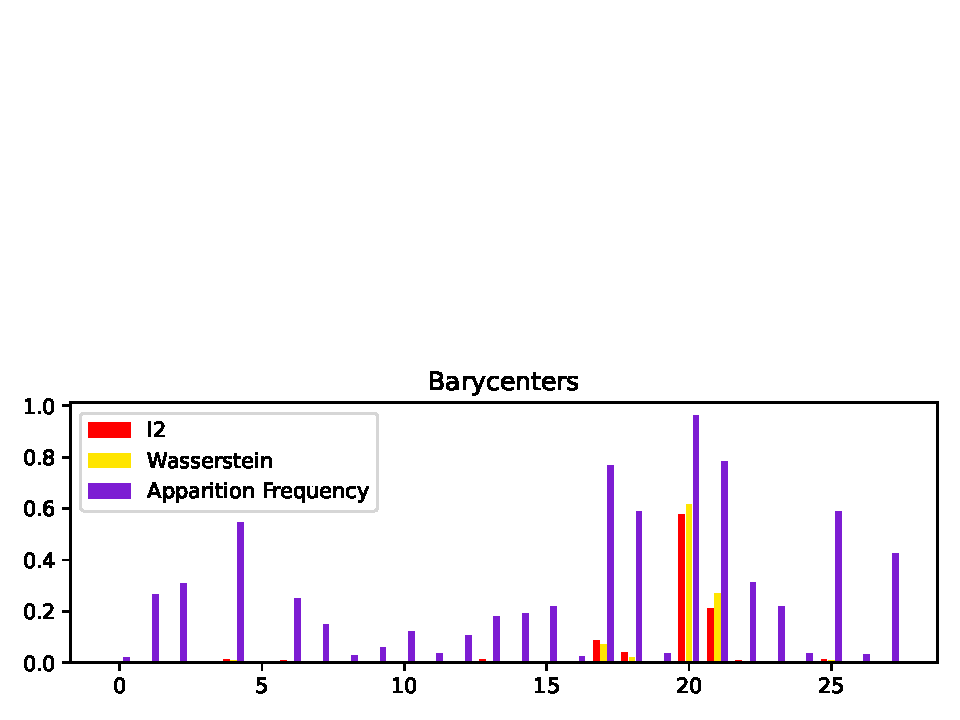
\includegraphics[width=\linewidth]{Images/Base_Nouns_Wasserstein_Barycenter_Acc.pdf}
    \caption{Representation of the uniform barycentre in red and the Wasserstein barycentre in yellow for the comparative \textsc{accusative} case.
    In purple is represented the proportion of treebanks that associate a given dependency relation with nouns in the accusative from the set of treebanks that inflect their nouns for case.}
    \label{fig:prototypes}
    % we need to know what the x means
\end{figure}

%Thus we show that there is a general structure for cases with the same name across languages, and that some of those can be quantitatively distinguished, but this method is not able to get visible distinctions. 

% en fait non, on a pas fait ça ^^, on a pas mis les distance entres les cas prototypique et les cas de chaque langue, ou potentiellement certains sont pas alignés avec leur nom....

% mais on le fait un peu avec le knn de la section suivante


\section{Case Clustering}

In this section we apply data visualisation techniques as a mean to look at the general landscape of case across languages.
This is a way to explore similarity between cases for many languages at once and without assuming a prototypical representation for each case.

From a practical annotation perspective, this is interesting since it is more likely too capture the underlying structure of UD's annotations.
Indeed, UD's guidelines are sometimes underspecified, which is expected from an annotation scheme whose aim is to be applicable to as many languages as possible.
Not all use cases and language specific phenomena will have been thought of during the creation of the guidelines.
Therefore, when annotators stumble upon a new structure that does not lend itself to a straightforward analysis, they will both turn to the guidelines and to other treebanks in order to see how similar phenomena might have been annotated in other languages.

We first used a t-SNE analysis \cite{tSNE} with the hope of seeing well defined clusters.
However, plotting all the cases at once proved unmanageable and so we resorted to visualising only a pair of cases each time.
%of finding two clusters, one for each case.

The algorithm consists in looking at the probability distribution generated by the high dimensional vectors representing each instance of the cases and generating a distribution over pairs of those vectors in a way that pairs of \emph{close} vectors are assigned higher probabilities.
Then t-SNE defines a probability distribution on pairs of 2D points that minimizes the Kullback-Leibler divergence between the two distributions.


\begin{figure}[h]
    \begin{center}
    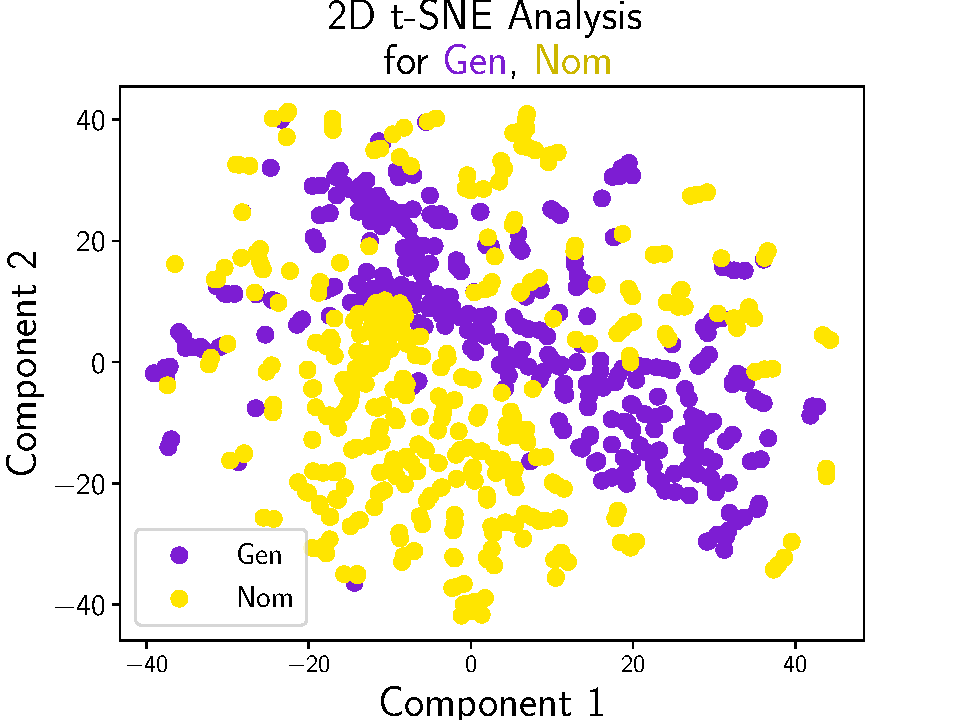
\includegraphics[width=.9\linewidth]{Images/tsne_Gen_Nom.pdf}
    \end{center}
    \caption{Representation of 2D t-SNE analysis of \scsf{genitive} and \scsf{nominative} profiles gathered on all the words marked for these cases.}
    \label{fig:tsne1}
\end{figure}

\begin{figure}[h]
    \begin{center}
    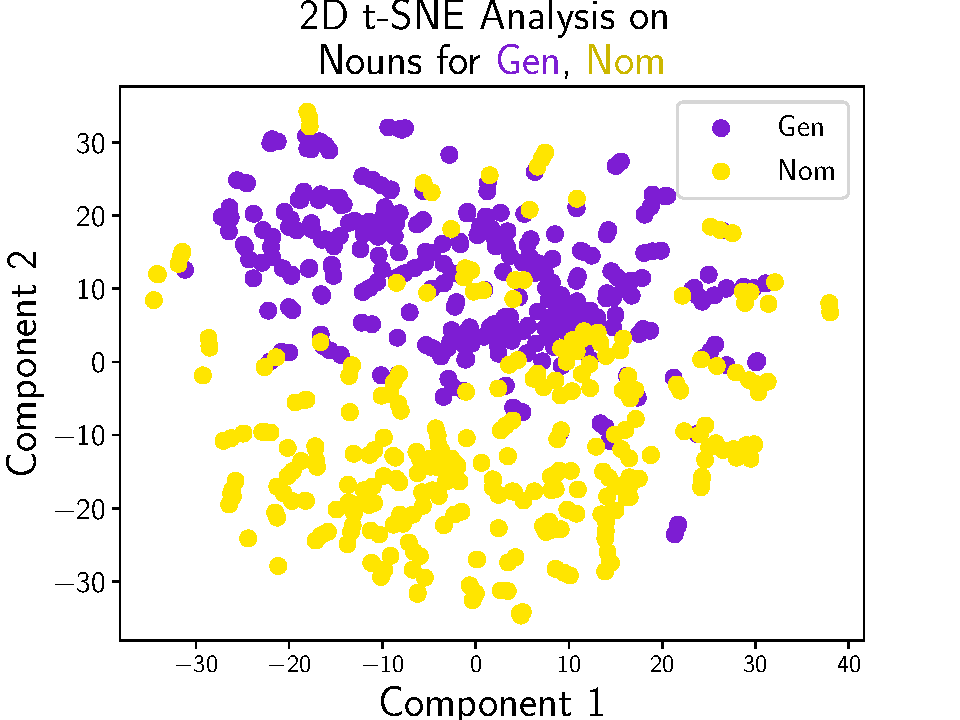
\includegraphics[width=.9\linewidth]{Images/tsne_Gen_Nom_Nouns.pdf}
    \end{center}
    \caption{Representation of 2D t-SNE analysis of \scsf{genitive} and \scsf{nominative} profiles gathered only on the nouns inflected for these cases.}
\label{fig:tsne2}
\end{figure}

Figures \ref{fig:tsne1} and \ref{fig:tsne2} represents the t-SNE applied to all the \scsf{nominatives} and \scsf{genitives} using either the profiles computed on all the words, or just on nouns.
It seems that the two cases make for clusters, in the sense they can be grouped along distinct directions.
While this is not enough for us to have a classification algorithm, it hints towards possible ways to visualise the difference between cases.

To confirm this hunch we tried to use ToMATo \cite{ToMATo}, a persistence based clustering algorithm, which uses sub-level sets of a function to design a persistence diagram and derive clusters.
The implementation that was used comes from \newcite{Gudhi}.
The idea behind ToMATo is to compute the density at each point in the representation space and to cluster points using geodesics: every point above a certain elevation and inside the same geodesic belongs in the same cluster (the same hill) and every point below is ignored.

By repeating the process for different elevations we can see clusters appear and merge.
When two clusters merge, the one with the highest elevation absorbs the other and we say that the lowest one dies.
One can then represent on a diagram the birth and death time of each cluster.
This is depicted on figure \ref{fig:tomato1} for \scsf{genitives} and \scsf{nominatives}.
The closer a cluster is to the diagonal the shorter its life and therefore the more likely it is to represent random noise rather than an actual cluster.
%So there seems to be two or three clusters.

\begin{figure}[h]
  \centering
  \vspace*{-12pt}
  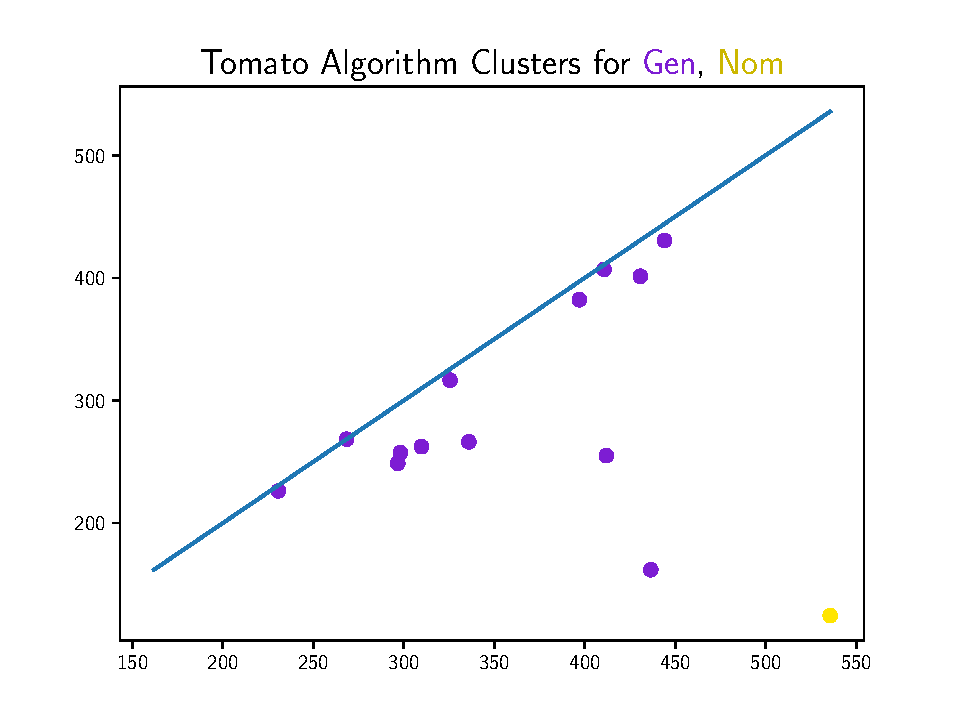
\includegraphics[width=\linewidth]{Images/tomato_Gen_Nom_Nouns.pdf}
  \caption{Representation of the ToMATo algorithm for \scsf{genitive} and \scsf{nominative} profiles.}
  \label{fig:tomato1}
\end{figure}

In figure \ref{fig:tomato1} the algorithm proposes multiple clusters, which couldn't be combined to form better defined clusters.
This suggests, as already suggested by figures \ref{fig:tsne1} and \ref{fig:tsne2} that the possible clusters are not well defined and might overlap with each other.
To try and measure the overlap of the clusters, we computed a confusion matrix by the method of the $k$-nearest neighbours.

\begin{table}[h]
	\centering
	\pgfplotsset{colormap={CM}{rgb255=(125, 29, 211) color=(pink) rgb255=(255, 229, 0)}, width=\linewidth}
% \pgfplotstabletypeset[
% 	color cells={min=0, max=250},
% 	col sep=comma,
%   every columns/.style ={},
%   display columns/0/.style={column name={Acc}},
%   display columns/1/.style={column name={Gen}},
%   display columns/2/.style={column name={Loc}},
%   display columns/3/.style={column name={Nom}},
% ]{
% 	130, 62, 51, 34
% 	69, 156, 16, 42
% 	35, 57, 29, 34
% 	29, 28, 9, 227
% }
\begin{tabular}{|c|cccc|}%
    \hline
  \diagbox{Pred.}{Target} & Acc & Gen & Loc & Nom\\%
  \hline
  Acc & \cellcolor [rgb]{0.99998, 0.75583, 0.72043}\definecolor {mapped color}{rgb}{0.99998, 0.75583, 0.72043}\pgfutilensuremath {130}&\cellcolor [rgb]{0.7429, 0.42914, 0.78905}\definecolor {mapped color}{rgb}{0.7429, 0.42914, 0.78905}\pgfutilensuremath {62}&\cellcolor [rgb]{0.69807, 0.37317, 0.79585}\definecolor {mapped color}{rgb}{0.69807, 0.37317, 0.79585}\pgfutilensuremath {51}&\cellcolor [rgb]{0.62877, 0.28668, 0.80638}\definecolor {mapped color}{rgb}{0.62877, 0.28668, 0.80638}\pgfutilensuremath {34}\\%
  Gen & \cellcolor [rgb]{0.77144, 0.46475, 0.78471}\definecolor {mapped color}{rgb}{0.77144, 0.46475, 0.78471}\pgfutilensuremath {69}&\cellcolor [rgb]{0.99998, 0.7866, 0.56451}\definecolor {mapped color}{rgb}{0.99998, 0.7866, 0.56451}\pgfutilensuremath {156}&\cellcolor [rgb]{0.5554, 0.19511, 0.81752}\definecolor {mapped color}{rgb}{0.5554, 0.19511, 0.81752}\pgfutilensuremath {16}&\cellcolor [rgb]{0.66138, 0.3274, 0.80142}\definecolor {mapped color}{rgb}{0.66138, 0.3274, 0.80142}\pgfutilensuremath {42}\\%
  Loc & \cellcolor [rgb]{0.63284, 0.29178, 0.80576}\definecolor {mapped color}{rgb}{0.63284, 0.29178, 0.80576}\pgfutilensuremath {35}&\cellcolor [rgb]{0.72253, 0.4037, 0.79214}\definecolor {mapped color}{rgb}{0.72253, 0.4037, 0.79214}\pgfutilensuremath {57}&\cellcolor [rgb]{0.6084, 0.26125, 0.80948}\definecolor {mapped color}{rgb}{0.6084, 0.26125, 0.80948}\pgfutilensuremath {29}&\cellcolor [rgb]{0.62877, 0.28668, 0.80638}\definecolor {mapped color}{rgb}{0.62877, 0.28668, 0.80638}\pgfutilensuremath {34}\\%
  Nom & \cellcolor [rgb]{0.6084, 0.26125, 0.80948}\definecolor {mapped color}{rgb}{0.6084, 0.26125, 0.80948}\pgfutilensuremath {29}&\cellcolor [rgb]{0.60431, 0.25616, 0.81009}\definecolor {mapped color}{rgb}{0.60431, 0.25616, 0.81009}\pgfutilensuremath {28}&\cellcolor [rgb]{0.52687, 0.1595, 0.82185}\definecolor {mapped color}{rgb}{0.52687, 0.1595, 0.82185}\pgfutilensuremath {9}&\cellcolor [rgb]{0.99998, 0.87062, 0.13875}\definecolor {mapped color}{rgb}{0.99998, 0.87062, 0.13875}\pgfutilensuremath {227}\\%
  \hline
\end{tabular}%

\medskip

\pgfplotscolorbardrawstandalone[%
  colorbar style={
    ticklabel style={
      font=\tiny,
      /pgf/number format/precision=3,
      /pgf/number format/relative*=4,
    },
  },
  colorbar horizontal,
  colormap access=const,
   point meta min=0, point meta max=250]
	\caption{Confusion matrix for $k$-NN with $k = 11$ on \texttt{Acc, Gen, Loc, Nom}.
 Rows correspond to the prediction and columns to the expected value.}
	\label{tab:knn}
\end{table}

As we can see in table \ref{tab:knn}, while cases that are present in many languages (\scsf{Nominative, Accusative, Genitive}) are quite recognisable, it is definitely not obvious, especially when throwing on other less common cases such as locative.
In fact, changing the parameter $k$ does not lead to significantly better results.
The more common cases are less recognisable with decreasing $k$, leading to a worse classification, and the less common cases are even more blurred when increasing $k$, since they are flooded in the total number of samples.
Moreover, whatever the parameter, there are always samples from common core cases that are classified as other cases.
It appears that the portion of space occupied by each case is neither fully distinct from the others, causing confusion when trying to cluster cases with the same names as well as limiting our ability to distinguish smaller cases from ones that take more space, nor is it well connected, given the fact some samples are always closer to other cases.% leading us to interrogations on the shape of the portion of space occupied.

%\section{The \texttt{Case} Feature across Treebanks}
While realising this study, we stumbled upon a number of incongruities in the way the different corpus use the \texttt{Case} feature.

There are essentially three ways the feature \texttt{Case} is used in the UD treebanks.
The first and by far the most common use is to annotate inflected forms of nouns, pronouns and proper nouns in languages where these words inflect according to their role in a clause, as well as determiners, adjectives and participles in languages where they inflect to match the case of their governor.

The second use that is documented in UD's guidelines\footnote{See the page of the \texttt{Case} feature: \url{https://universaldependencies.org/u/feat/Case.html}.}, is to annotate adpositions with the case they give to their nominal phrase, especially so in languages without over case marking on nouns.
This annotation principle indicates that UD leans more toward the application of comparative concepts to individual languages.
Indeed, if a language does not use the case category, then the ``case'' represented by an adposition can only be inferred either by comparing its distribution to the distribution of actual cases in languages that possess that category, or by applying formal comparative definitions.

However, this is not always how this feature is used, as in Czech CLTT treebank \cite{cltt} for example, adpositions are annotated with the \texttt{Case} feature and their value always match that of their governing noun.
This is all the more surprising that Czech adpositions are invariable and can license several case values.

This indeed points to another problem with case annotation on adpositions.
Like languages exhibiting case syncretism\footnote{A given word form can be ambiguous as to its morphological features. For example, the Latin form \textit{rosae} can be either a genitive or dative singular or a nominative or vocative plural.}, adpositions can in principle also be used to mark different syntactic and semantic roles.
It becomes then even less clear how one should proceed in assigning cases to adposition.

The third and most divergent use of the \texttt{Case} feature can be seen in the Persian Seraji treebank.
In this treebank, we only find three case values : \texttt{Case=Loc}, \texttt{Case=Tem} and \texttt{Case=Voc}.
The first two values are exclusively used to annotate adverbs of place and adverbs of time respectively.
The third value is used to annotate an interjection used to create vocative noun phrase.

%Following on this method, we defined the vector spaces generated by the family of the vectors representing all the cases in a corpus (called \emph{case spaces}) and computing the cosine distance between two vectors, but this didn't yield any usable results. 
%Indeed the results were too blended in the number of results. 
%Moreover the density of data combined with the numerical precision needed for comparisons makes the results difficult to exploit manually. 
%We thus tried the following: computing the cosine distance between a vector and its projection on a case space. 
%This got us an aberration when looking at the projection of farsi vocative on arabic. 
%Indeed, farsi vocative was near orthogonal to arabic, while the two languages are close. 
%This actually comes from the fact that vocative in farsi is used to annotate some interjections used as adpositions, with the relation \texttt{case}. 

\section{Adposition Annotation}

As discussed in section 2, some corpora in UD make use of the \texttt{Case} feature on adpositions and it is recommended by UD's guidelines.

Given the postulate according to which all natural languages are equally expressive, one could indeed see case marking and the use of adpositions as two means of achieving the same linguistic goals.
Two means that are by no mean exclusive since languages that use case tend to have a rather limited inventory and use adpositions to express a broader range of meanings and relations.

Following \newcite{morphenglish}, we have applied the methods described above to represent certain adpositions and to give them a syntactically equivalent case representation.
This could partially prove the postulate, as well as help justifying the way some corpora annotate adpositions for case.

To do so, we counted the dependency relations leading to the governors of each adposition.
This gave us a distribution on syntactic usage of adpositions similar to a profile, and allowed us to compare adpositions to cases.

\begin{table}[h]
    \centering
    \renewcommand{\arraystretch}{1.3}
    \addtolength{\tabcolsep}{-.3ex}
    \begin{NiceTabular}{>{\sc}rcccccc}
    \bf Adpos & \tt advcl & \tt nmod & \tt nsubj & \tt obj & \tt obl\\
    À     & 16.7   & 17.3   & 0.04   & 0.38  & 63.4\\
    Dans   & 0.46   & 13.8   &      & 0.19  & 78.7\\
    Par    & 0.26   & 13.7   & 0.10   & 0.18  & 74.6\\
    Pour   & 29.5   & 15.9   &      & 0.02  & 41.2\\
    En    & 8.13   & 17.1   &      & 0.36  & 54.1\\
    Vers   & 0.26   & 35.7   &      &     & 62.1\\
    Avec   & 0.61   & 32.4   &      &     & 62.6\\
    De    & 2.10   & 68.0   & 0.14   & 1.31  & 14.3\\
    Sans   & 24.4   & 21.1   &      & 0.78  & 43.8\\
    Sous   & 0.21   & 22.9   & 0.02   & 72.8  &   \\
    Sur    & 0.47   & 36.3   &      & 0.10  & 59.4\\
    Sauf   & 10.7   & 22.6   &      &     & 38.1\\
    \CodeAfter
    \begin{tikzpicture}
        \draw[black] (1|-2) -- (7|-2);
        \foreach \i in {3, ..., 13} {\draw[black] (1|-\i) -- (7|-\i);}
        \draw[black, dashed] (2|-1) -- (2|-14);
    \end{tikzpicture}
    \end{NiceTabular}
    \caption{Dependency relation profiles of the governors irrespective of its part-of-speech of a few French adpositions.}
    \addtolength{\tabcolsep}{.3ex}
    \label{tab:adpos_fr}
\end{table}

Table \ref{tab:adpos_fr} represents the uniform means of the representations of a few French adpositions across all French corpora.
As we can see, and could be predicted by French speakers, most adpositions are used in a similar way in French, mainly as \textsc{locatives} (\textsl{dans, par, sur, sous, vers\ldots}) or \textsc{instrumentals/comitative} (\textsl{avec}).
For the other adpositions, we see that there is a non-negligible proportion of usage that leads to \texttt{advcl}.
This comes from infinitive constructions marking goal (\textsl{pour}), intent (\textsl{à}), avoidance (\textsl{sans}) or gerundive constructions marking manner (\textsl{en}).% is used before a verb, creating an adverbial clause.

This justifies the idea of giving a case to adpositions as a reasonable supposition, and confirms our postulate that adpositions replace some cases in language without cases (French actually has cases on personal pronouns; but not for any of the cases \textit{replaced} by adpositions).
We believe that this method could be extended to any other part of speech with adequate semantics and syntactic constructions.

% \section{Parsing ? }

\section{Conclusion}

In this paper, we have investigated the comparative-descriptive confusion that Haspelmath warned us about using Universal Dependency data.
We have compared cases between different languages as is it was a commensurable descriptive category and seen that at least for some closely related languages the alignment stands at least for core cases.
We then tried to represent archetypal cases as if case was a comparative concept applied onto each treebank, and saw that core cases mostly align with our expectations.
However, this asks for a more principled analysis of the use of the term \textit{nominative} for the default case especially so when the nominative-accusative distinction does not exist or when it does not simply mark a syntactic role but also definiteness for example.




\bibliographystyle{acl_natbib}
\bibliography{main}

%\newpage

\section*{Appendix}
\begin{table}[h]
	\centering
    \setlength\tabcolsep{3.5pt}\renewcommand\arraystretch{1.25}
	\pgfplotsset{colormap={CM}{rgb255=(125, 29, 211) color=(pink) rgb255=(255,229,0)}, width=\linewidth}


\resizebox{\linewidth}{!}{
\begin{tabular}{|c|ccccccc|}%
\hline
\diagbox{ Cs }{Ru} & Acc & Dat & Gen & Ins & Loc & Nom &Par\\%
\hline
Acc & \cellcolor [rgb]{0.64049,0.3013,0.8046}\definecolor {mapped color}{rgb}{0.64049,0.3013,0.8046}\pgfutilensuremath {0.3}&\cellcolor [rgb]{0.7215,0.40242,0.7923}\definecolor {mapped color}{rgb}{0.7215,0.40242,0.7923}\pgfutilensuremath {0.45}&\cellcolor [rgb]{0.74188,0.42786,0.7892}\definecolor {mapped color}{rgb}{0.74188,0.42786,0.7892}\pgfutilensuremath {0.49}&\cellcolor [rgb]{0.6247,0.28159,0.80699}\definecolor {mapped color}{rgb}{0.6247,0.28159,0.80699}\pgfutilensuremath {0.26}&\cellcolor [rgb]{0.74953,0.4374,0.78804}\definecolor {mapped color}{rgb}{0.74953,0.4374,0.78804}\pgfutilensuremath {0.51}&\cellcolor [rgb]{0.70113,0.37698,0.7954}\definecolor {mapped color}{rgb}{0.70113,0.37698,0.7954}\pgfutilensuremath {0.41}&\cellcolor [rgb]{0.99998,0.75404,0.72943}\definecolor {mapped color}{rgb}{0.99998,0.75404,0.72943}\pgfutilensuremath {1.03}\\%
Dat & \cellcolor [rgb]{0.73883,0.42404,0.78966}\definecolor {mapped color}{rgb}{0.73883,0.42404,0.78966}\pgfutilensuremath {0.49}&\cellcolor [rgb]{0.7159,0.39543,0.79315}\definecolor {mapped color}{rgb}{0.7159,0.39543,0.79315}\pgfutilensuremath {0.44}&\cellcolor [rgb]{0.76787,0.46028,0.78523}\definecolor {mapped color}{rgb}{0.76787,0.46028,0.78523}\pgfutilensuremath {0.55}&\cellcolor [rgb]{0.68584,0.3579,0.79771}\definecolor {mapped color}{rgb}{0.68584,0.3579,0.79771}\pgfutilensuremath {0.38}&\cellcolor [rgb]{0.72557,0.4075,0.79167}\definecolor {mapped color}{rgb}{0.72557,0.4075,0.79167}\pgfutilensuremath {0.46}&\cellcolor [rgb]{0.75005,0.43803,0.78795}\definecolor {mapped color}{rgb}{0.75005,0.43803,0.78795}\pgfutilensuremath {0.51}&\cellcolor [rgb]{0.96048,0.70067,0.756}\definecolor {mapped color}{rgb}{0.96048,0.70067,0.756}\pgfutilensuremath {0.92}\\%
Gen & \cellcolor [rgb]{0.74596,0.43294,0.78857}\definecolor {mapped color}{rgb}{0.74596,0.43294,0.78857}\pgfutilensuremath {0.5}&\cellcolor [rgb]{0.69603,0.3706,0.79616}\definecolor {mapped color}{rgb}{0.69603,0.3706,0.79616}\pgfutilensuremath {0.4}&\cellcolor [rgb]{0.59004,0.23836,0.81226}\definecolor {mapped color}{rgb}{0.59004,0.23836,0.81226}\pgfutilensuremath {0.2}&\cellcolor [rgb]{0.65373,0.31783,0.80258}\definecolor {mapped color}{rgb}{0.65373,0.31783,0.80258}\pgfutilensuremath {0.32}&\cellcolor [rgb]{0.72711,0.40941,0.79143}\definecolor {mapped color}{rgb}{0.72711,0.40941,0.79143}\pgfutilensuremath {0.47}&\cellcolor [rgb]{0.75717,0.44691,0.78687}\definecolor {mapped color}{rgb}{0.75717,0.44691,0.78687}\pgfutilensuremath {0.52}&\cellcolor [rgb]{0.99998,0.75671,0.71593}\definecolor {mapped color}{rgb}{0.99998,0.75671,0.71593}\pgfutilensuremath {1.05}\\%
Ins & \cellcolor [rgb]{0.70673,0.38397,0.79453}\definecolor {mapped color}{rgb}{0.70673,0.38397,0.79453}\pgfutilensuremath {0.43}&\cellcolor [rgb]{0.6894,0.36235,0.79716}\definecolor {mapped color}{rgb}{0.6894,0.36235,0.79716}\pgfutilensuremath {0.39}&\cellcolor [rgb]{0.73016,0.41322,0.79097}\definecolor {mapped color}{rgb}{0.73016,0.41322,0.79097}\pgfutilensuremath {0.47}&\cellcolor [rgb]{0.63489,0.2943,0.80544}\definecolor {mapped color}{rgb}{0.63489,0.2943,0.80544}\pgfutilensuremath {0.28}&\cellcolor [rgb]{0.70215,0.37827,0.79523}\definecolor {mapped color}{rgb}{0.70215,0.37827,0.79523}\pgfutilensuremath {0.42}&\cellcolor [rgb]{0.7164,0.39604,0.79306}\definecolor {mapped color}{rgb}{0.7164,0.39604,0.79306}\pgfutilensuremath {0.44}&\cellcolor [rgb]{0.9722,0.7153,0.75421}\definecolor {mapped color}{rgb}{0.9722,0.7153,0.75421}\pgfutilensuremath {0.95}\\%
Loc & \cellcolor [rgb]{0.75922,0.44948,0.78656}\definecolor {mapped color}{rgb}{0.75922,0.44948,0.78656}\pgfutilensuremath {0.53}&\cellcolor [rgb]{0.73221,0.41577,0.79066}\definecolor {mapped color}{rgb}{0.73221,0.41577,0.79066}\pgfutilensuremath {0.48}&\cellcolor [rgb]{0.76685,0.45901,0.7854}\definecolor {mapped color}{rgb}{0.76685,0.45901,0.7854}\pgfutilensuremath {0.54}&\cellcolor [rgb]{0.70827,0.38588,0.7943}\definecolor {mapped color}{rgb}{0.70827,0.38588,0.7943}\pgfutilensuremath {0.43}&\cellcolor [rgb]{0.74596,0.43294,0.78857}\definecolor {mapped color}{rgb}{0.74596,0.43294,0.78857}\pgfutilensuremath {0.5}&\cellcolor [rgb]{0.77194,0.46536,0.78462}\definecolor {mapped color}{rgb}{0.77194,0.46536,0.78462}\pgfutilensuremath {0.55}&\cellcolor [rgb]{0.9773,0.72165,0.75343}\definecolor {mapped color}{rgb}{0.9773,0.72165,0.75343}\pgfutilensuremath {0.96}\\%
Nom & \cellcolor [rgb]{0.74188,0.42786,0.7892}\definecolor {mapped color}{rgb}{0.74188,0.42786,0.7892}\pgfutilensuremath {0.49}&\cellcolor [rgb]{0.76941,0.46219,0.785}\definecolor {mapped color}{rgb}{0.76941,0.46219,0.785}\pgfutilensuremath {0.55}&\cellcolor [rgb]{0.78978,0.48764,0.78192}\definecolor {mapped color}{rgb}{0.78978,0.48764,0.78192}\pgfutilensuremath {0.59}&\cellcolor [rgb]{0.68431,0.356,0.79794}\definecolor {mapped color}{rgb}{0.68431,0.356,0.79794}\pgfutilensuremath {0.38}&\cellcolor [rgb]{0.7913,0.48953,0.78168}\definecolor {mapped color}{rgb}{0.7913,0.48953,0.78168}\pgfutilensuremath {0.59}&\cellcolor [rgb]{0.61807,0.27333,0.808}\definecolor {mapped color}{rgb}{0.61807,0.27333,0.808}\pgfutilensuremath {0.25}&\cellcolor [rgb]{0.99998,0.76617,0.66795}\definecolor {mapped color}{rgb}{0.99998,0.76617,0.66795}\pgfutilensuremath {1.11}\\%
\hline
\end{tabular}
}
\caption{Distances between Czech CLTT and Russian GSD case profiles.}

\medskip

% ['Acc', 'Dat', 'Gen', 'Ins', 'Loc', 'Nom'] 
\resizebox{\linewidth}{!}{
\begin{tabular}{|c|ccccccc|}%
\hline
\diagbox{ Cs }{Ru} & Acc & Dat & Gen & Ins & Loc & Nom & Par\\%
\hline
Acc&\cellcolor [rgb]{0.6196,0.27524,0.80777}\definecolor {mapped color}{rgb}{0.6196,0.27524,0.80777}\pgfutilensuremath {0.25}&\cellcolor [rgb]{0.81169,0.51497,0.77858}\definecolor {mapped color}{rgb}{0.81169,0.51497,0.77858}\pgfutilensuremath {0.63}&\cellcolor [rgb]{0.84837,0.56076,0.77301}\definecolor {mapped color}{rgb}{0.84837,0.56076,0.77301}\pgfutilensuremath {0.7}&\cellcolor [rgb]{0.70163,0.37761,0.7953}\definecolor {mapped color}{rgb}{0.70163,0.37761,0.7953}\pgfutilensuremath {0.42}&\cellcolor [rgb]{0.88863,0.61101,0.7669}\definecolor {mapped color}{rgb}{0.88863,0.61101,0.7669}\pgfutilensuremath {0.78}&\cellcolor [rgb]{0.88507,0.60655,0.76744}\definecolor {mapped color}{rgb}{0.88507,0.60655,0.76744}\pgfutilensuremath {0.78}&\cellcolor [rgb]{0.99998,0.75449,0.72717}\definecolor {mapped color}{rgb}{0.99998,0.75449,0.72717}\pgfutilensuremath {1.03}\\%
Dat&\cellcolor [rgb]{0.83055,0.53851,0.77573}\definecolor {mapped color}{rgb}{0.83055,0.53851,0.77573}\pgfutilensuremath {0.67}&\cellcolor [rgb]{0.67462,0.3439,0.79941}\definecolor {mapped color}{rgb}{0.67462,0.3439,0.79941}\pgfutilensuremath {0.36}&\cellcolor [rgb]{0.81474,0.5188,0.77812}\definecolor {mapped color}{rgb}{0.81474,0.5188,0.77812}\pgfutilensuremath {0.64}&\cellcolor [rgb]{0.72609,0.40814,0.7916}\definecolor {mapped color}{rgb}{0.72609,0.40814,0.7916}\pgfutilensuremath {0.46}&\cellcolor [rgb]{0.71387,0.39287,0.79344}\definecolor {mapped color}{rgb}{0.71387,0.39287,0.79344}\pgfutilensuremath {0.44}&\cellcolor [rgb]{0.91309,0.64153,0.76318}\definecolor {mapped color}{rgb}{0.91309,0.64153,0.76318}\pgfutilensuremath {0.83}&\cellcolor [rgb]{0.85501,0.56903,0.772}\definecolor {mapped color}{rgb}{0.85501,0.56903,0.772}\pgfutilensuremath {0.72}\\%
Gen&\cellcolor [rgb]{0.95741,0.69685,0.75645}\definecolor {mapped color}{rgb}{0.95741,0.69685,0.75645}\pgfutilensuremath {0.92}&\cellcolor [rgb]{0.81017,0.51308,0.77882}\definecolor {mapped color}{rgb}{0.81017,0.51308,0.77882}\pgfutilensuremath {0.63}&\cellcolor [rgb]{0.53604,0.17094,0.82047}\definecolor {mapped color}{rgb}{0.53604,0.17094,0.82047}\pgfutilensuremath {0.09}&\cellcolor [rgb]{0.81628,0.5207,0.7779}\definecolor {mapped color}{rgb}{0.81628,0.5207,0.7779}\pgfutilensuremath {0.64}&\cellcolor [rgb]{0.90596,0.63263,0.76428}\definecolor {mapped color}{rgb}{0.90596,0.63263,0.76428}\pgfutilensuremath {0.82}&\cellcolor [rgb]{0.99998,0.75154,0.74217}\definecolor {mapped color}{rgb}{0.99998,0.75154,0.74217}\pgfutilensuremath {1.01}&\cellcolor [rgb]{0.99998,0.7749,0.62373}\definecolor {mapped color}{rgb}{0.99998,0.7749,0.62373}\pgfutilensuremath {1.17}\\%
Ins&\cellcolor [rgb]{0.82086,0.52641,0.77719}\definecolor {mapped color}{rgb}{0.82086,0.52641,0.77719}\pgfutilensuremath {0.65}&\cellcolor [rgb]{0.7052,0.38206,0.79477}\definecolor {mapped color}{rgb}{0.7052,0.38206,0.79477}\pgfutilensuremath {0.42}&\cellcolor [rgb]{0.81322,0.51688,0.77835}\definecolor {mapped color}{rgb}{0.81322,0.51688,0.77835}\pgfutilensuremath {0.63}&\cellcolor [rgb]{0.69705,0.37189,0.79599}\definecolor {mapped color}{rgb}{0.69705,0.37189,0.79599}\pgfutilensuremath {0.41}&\cellcolor [rgb]{0.77042,0.46347,0.78485}\definecolor {mapped color}{rgb}{0.77042,0.46347,0.78485}\pgfutilensuremath {0.55}&\cellcolor [rgb]{0.87386,0.59256,0.76913}\definecolor {mapped color}{rgb}{0.87386,0.59256,0.76913}\pgfutilensuremath {0.75}&\cellcolor [rgb]{0.90901,0.63644,0.76381}\definecolor {mapped color}{rgb}{0.90901,0.63644,0.76381}\pgfutilensuremath {0.82}\\%
Loc&\cellcolor [rgb]{0.82391,0.53024,0.77673}\definecolor {mapped color}{rgb}{0.82391,0.53024,0.77673}\pgfutilensuremath {0.66}&\cellcolor [rgb]{0.61807,0.27333,0.808}\definecolor {mapped color}{rgb}{0.61807,0.27333,0.808}\pgfutilensuremath {0.25}&\cellcolor [rgb]{0.73985,0.42532,0.7895}\definecolor {mapped color}{rgb}{0.73985,0.42532,0.7895}\pgfutilensuremath {0.49}&\cellcolor [rgb]{0.70113,0.37698,0.7954}\definecolor {mapped color}{rgb}{0.70113,0.37698,0.7954}\pgfutilensuremath {0.41}&\cellcolor [rgb]{0.67462,0.3439,0.79941}\definecolor {mapped color}{rgb}{0.67462,0.3439,0.79941}\pgfutilensuremath {0.36}&\cellcolor [rgb]{0.91666,0.64598,0.76265}\definecolor {mapped color}{rgb}{0.91666,0.64598,0.76265}\pgfutilensuremath {0.84}&\cellcolor [rgb]{0.85092,0.56395,0.77263}\definecolor {mapped color}{rgb}{0.85092,0.56395,0.77263}\pgfutilensuremath {0.71}\\%
Nom&\cellcolor [rgb]{0.90494,0.63135,0.76443}\definecolor {mapped color}{rgb}{0.90494,0.63135,0.76443}\pgfutilensuremath {0.81}&\cellcolor [rgb]{0.90799,0.63516,0.76396}\definecolor {mapped color}{rgb}{0.90799,0.63516,0.76396}\pgfutilensuremath {0.82}&\cellcolor [rgb]{0.962,0.70258,0.75575}\definecolor {mapped color}{rgb}{0.962,0.70258,0.75575}\pgfutilensuremath {0.93}&\cellcolor [rgb]{0.83513,0.54424,0.77502}\definecolor {mapped color}{rgb}{0.83513,0.54424,0.77502}\pgfutilensuremath {0.68}&\cellcolor [rgb]{0.97882,0.72356,0.7532}\definecolor {mapped color}{rgb}{0.97882,0.72356,0.7532}\pgfutilensuremath {0.96}&\cellcolor [rgb]{0.57935,0.22499,0.81387}\definecolor {mapped color}{rgb}{0.57935,0.22499,0.81387}\pgfutilensuremath {0.18}&\cellcolor [rgb]{0.99998,0.77373,0.62973}\definecolor {mapped color}{rgb}{0.99998,0.77373,0.62973}\pgfutilensuremath {1.16}\\%
\hline
\end{tabular}}
\caption{Distances between Czech CLTT and Russian GSD noun case profiles.}

\medskip

\resizebox{\linewidth}{!}{
% ['Acc', 'Dat', 'Gen', 'Ins', 'Loc', 'Nom'] 
\begin {tabular}{|c|cccccc|}%
\hline
&Acc&Dat&Gen&Ins&Loc&Nom\\%
\hline
Acc&\cellcolor [rgb]{0.49019,0.11372,0.82744}\definecolor {mapped color}{rgb}{0.49019,0.11372,0.82744}\pgfutilensuremath {0}&\cellcolor [rgb]{0.6522,0.31593,0.80281}\definecolor {mapped color}{rgb}{0.6522,0.31593,0.80281}\pgfutilensuremath {0.32}&\cellcolor [rgb]{0.67921,0.34964,0.79872}\definecolor {mapped color}{rgb}{0.67921,0.34964,0.79872}\pgfutilensuremath {0.37}&\cellcolor [rgb]{0.62267,0.27905,0.8073}\definecolor {mapped color}{rgb}{0.62267,0.27905,0.8073}\pgfutilensuremath {0.26}&\cellcolor [rgb]{0.66953,0.33755,0.80019}\definecolor {mapped color}{rgb}{0.66953,0.33755,0.80019}\pgfutilensuremath {0.35}&\cellcolor [rgb]{0.68227,0.35344,0.79825}\definecolor {mapped color}{rgb}{0.68227,0.35344,0.79825}\pgfutilensuremath {0.38}\\%
Dat &\cellcolor [rgb]{0.6522,0.31593,0.80281}\definecolor {mapped color}{rgb}{0.6522,0.31593,0.80281}\pgfutilensuremath {0.32}&\cellcolor [rgb]{0.49019,0.11372,0.82744}\definecolor {mapped color}{rgb}{0.49019,0.11372,0.82744}\pgfutilensuremath {0}&\cellcolor [rgb]{0.6894,0.36235,0.79716}\definecolor {mapped color}{rgb}{0.6894,0.36235,0.79716}\pgfutilensuremath {0.39}&\cellcolor [rgb]{0.57883,0.22437,0.81396}\definecolor {mapped color}{rgb}{0.57883,0.22437,0.81396}\pgfutilensuremath {0.17}&\cellcolor [rgb]{0.5656,0.20782,0.81596}\definecolor {mapped color}{rgb}{0.5656,0.20782,0.81596}\pgfutilensuremath {0.15}&\cellcolor [rgb]{0.75105,0.4393,0.7878}\definecolor {mapped color}{rgb}{0.75105,0.4393,0.7878}\pgfutilensuremath {0.51}\\%
Gen &\cellcolor [rgb]{0.67921,0.34964,0.79872}\definecolor {mapped color}{rgb}{0.67921,0.34964,0.79872}\pgfutilensuremath {0.37}&\cellcolor [rgb]{0.6894,0.36235,0.79716}\definecolor {mapped color}{rgb}{0.6894,0.36235,0.79716}\pgfutilensuremath {0.39}&\cellcolor [rgb]{0.49019,0.11372,0.82744}\definecolor {mapped color}{rgb}{0.49019,0.11372,0.82744}\pgfutilensuremath {0}&\cellcolor [rgb]{0.65373,0.31783,0.80258}\definecolor {mapped color}{rgb}{0.65373,0.31783,0.80258}\pgfutilensuremath {0.32}&\cellcolor [rgb]{0.68584,0.3579,0.79771}\definecolor {mapped color}{rgb}{0.68584,0.3579,0.79771}\pgfutilensuremath {0.38}&\cellcolor [rgb]{0.74036,0.42595,0.78943}\definecolor {mapped color}{rgb}{0.74036,0.42595,0.78943}\pgfutilensuremath {0.49}\\%
Ins &\cellcolor [rgb]{0.62267,0.27905,0.8073}\definecolor {mapped color}{rgb}{0.62267,0.27905,0.8073}\pgfutilensuremath {0.26}&\cellcolor [rgb]{0.57883,0.22437,0.81396}\definecolor {mapped color}{rgb}{0.57883,0.22437,0.81396}\pgfutilensuremath {0.17}&\cellcolor [rgb]{0.65373,0.31783,0.80258}\definecolor {mapped color}{rgb}{0.65373,0.31783,0.80258}\pgfutilensuremath {0.32}&\cellcolor [rgb]{0.49019,0.11372,0.82744}\definecolor {mapped color}{rgb}{0.49019,0.11372,0.82744}\pgfutilensuremath {0}&\cellcolor [rgb]{0.62317,0.27968,0.80722}\definecolor {mapped color}{rgb}{0.62317,0.27968,0.80722}\pgfutilensuremath {0.26}&\cellcolor [rgb]{0.69705,0.37189,0.79599}\definecolor {mapped color}{rgb}{0.69705,0.37189,0.79599}\pgfutilensuremath {0.41}\\%
Loc &\cellcolor [rgb]{0.66953,0.33755,0.80019}\definecolor {mapped color}{rgb}{0.66953,0.33755,0.80019}\pgfutilensuremath {0.35}&\cellcolor [rgb]{0.5656,0.20782,0.81596}\definecolor {mapped color}{rgb}{0.5656,0.20782,0.81596}\pgfutilensuremath {0.15}&\cellcolor [rgb]{0.68584,0.3579,0.79771}\definecolor {mapped color}{rgb}{0.68584,0.3579,0.79771}\pgfutilensuremath {0.38}&\cellcolor [rgb]{0.62317,0.27968,0.80722}\definecolor {mapped color}{rgb}{0.62317,0.27968,0.80722}\pgfutilensuremath {0.26}&\cellcolor [rgb]{0.49019,0.11372,0.82744}\definecolor {mapped color}{rgb}{0.49019,0.11372,0.82744}\pgfutilensuremath {0}&\cellcolor [rgb]{0.77501,0.4692,0.78416}\definecolor {mapped color}{rgb}{0.77501,0.4692,0.78416}\pgfutilensuremath {0.56}\\%
Nom &\cellcolor [rgb]{0.68227,0.35344,0.79825}\definecolor {mapped color}{rgb}{0.68227,0.35344,0.79825}\pgfutilensuremath {0.38}&\cellcolor [rgb]{0.75105,0.4393,0.7878}\definecolor {mapped color}{rgb}{0.75105,0.4393,0.7878}\pgfutilensuremath {0.51}&\cellcolor [rgb]{0.74036,0.42595,0.78943}\definecolor {mapped color}{rgb}{0.74036,0.42595,0.78943}\pgfutilensuremath {0.49}&\cellcolor [rgb]{0.69705,0.37189,0.79599}\definecolor {mapped color}{rgb}{0.69705,0.37189,0.79599}\pgfutilensuremath {0.41}&\cellcolor [rgb]{0.77501,0.4692,0.78416}\definecolor {mapped color}{rgb}{0.77501,0.4692,0.78416}\pgfutilensuremath {0.56}&\cellcolor [rgb]{0.49019,0.11372,0.82744}\definecolor {mapped color}{rgb}{0.49019,0.11372,0.82744}\pgfutilensuremath {0}\\%
\hline
\end{tabular}}
\caption{Distances between Czech CLTT case profiles.}

\end{table}

\begin{table}
	\centering
    \setlength\tabcolsep{3.5pt}\renewcommand\arraystretch{1.25}
	\pgfplotsset{colormap={CM}{rgb255=(125, 29, 211) color=(pink) rgb255=(255,229,0)}, width=\linewidth}

 \resizebox{\linewidth}{!}{
\begin{tabular}{|c|cccccc|}%
\hline
&Acc&Dat&Gen&Ins&Loc&Nom\\%
\hline
Acc& \cellcolor [rgb]{0.49019,0.11372,0.82744}\definecolor {mapped color}{rgb}{0.49019,0.11372,0.82744}\pgfutilensuremath {0}&\cellcolor [rgb]{0.79997,0.50037,0.78038}\definecolor {mapped color}{rgb}{0.79997,0.50037,0.78038}\pgfutilensuremath {0.61}&\cellcolor [rgb]{0.8764,0.59573,0.76875}\definecolor {mapped color}{rgb}{0.8764,0.59573,0.76875}\pgfutilensuremath {0.76}&\cellcolor [rgb]{0.77194,0.46536,0.78462}\definecolor {mapped color}{rgb}{0.77194,0.46536,0.78462}\pgfutilensuremath {0.55}&\cellcolor [rgb]{0.79488,0.49399,0.78114}\definecolor {mapped color}{rgb}{0.79488,0.49399,0.78114}\pgfutilensuremath {0.6}&\cellcolor [rgb]{0.84991,0.56268,0.77278}\definecolor {mapped color}{rgb}{0.84991,0.56268,0.77278}\pgfutilensuremath {0.71}\\%
Dat& \cellcolor [rgb]{0.79997,0.50037,0.78038}\definecolor {mapped color}{rgb}{0.79997,0.50037,0.78038}\pgfutilensuremath {0.61}&\cellcolor [rgb]{0.49019,0.11372,0.82744}\definecolor {mapped color}{rgb}{0.49019,0.11372,0.82744}\pgfutilensuremath {0}&\cellcolor [rgb]{0.81984,0.52515,0.77734}\definecolor {mapped color}{rgb}{0.81984,0.52515,0.77734}\pgfutilensuremath {0.65}&\cellcolor [rgb]{0.58392,0.23071,0.81319}\definecolor {mapped color}{rgb}{0.58392,0.23071,0.81319}\pgfutilensuremath {0.18}&\cellcolor [rgb]{0.63081,0.28923,0.80606}\definecolor {mapped color}{rgb}{0.63081,0.28923,0.80606}\pgfutilensuremath {0.28}&\cellcolor [rgb]{0.90494,0.63135,0.76443}\definecolor {mapped color}{rgb}{0.90494,0.63135,0.76443}\pgfutilensuremath {0.81}\\%
Gen & \cellcolor [rgb]{0.8764,0.59573,0.76875}\definecolor {mapped color}{rgb}{0.8764,0.59573,0.76875}\pgfutilensuremath {0.76}&\cellcolor [rgb]{0.81984,0.52515,0.77734}\definecolor {mapped color}{rgb}{0.81984,0.52515,0.77734}\pgfutilensuremath {0.65}&\cellcolor [rgb]{0.49019,0.11372,0.82744}\definecolor {mapped color}{rgb}{0.49019,0.11372,0.82744}\pgfutilensuremath {0}&\cellcolor [rgb]{0.82545,0.53215,0.7765}\definecolor {mapped color}{rgb}{0.82545,0.53215,0.7765}\pgfutilensuremath {0.66}&\cellcolor [rgb]{0.74341,0.42975,0.78896}\definecolor {mapped color}{rgb}{0.74341,0.42975,0.78896}\pgfutilensuremath {0.5}&\cellcolor [rgb]{0.98952,0.73692,0.75157}\definecolor {mapped color}{rgb}{0.98952,0.73692,0.75157}\pgfutilensuremath {0.98}\\%
Ins &\cellcolor [rgb]{0.77194,0.46536,0.78462}\definecolor {mapped color}{rgb}{0.77194,0.46536,0.78462}\pgfutilensuremath {0.55}&\cellcolor [rgb]{0.58392,0.23071,0.81319}\definecolor {mapped color}{rgb}{0.58392,0.23071,0.81319}\pgfutilensuremath {0.18}&\cellcolor [rgb]{0.82545,0.53215,0.7765}\definecolor {mapped color}{rgb}{0.82545,0.53215,0.7765}\pgfutilensuremath {0.66}&\cellcolor [rgb]{0.49019,0.11372,0.82744}\definecolor {mapped color}{rgb}{0.49019,0.11372,0.82744}\pgfutilensuremath {0}&\cellcolor [rgb]{0.65985,0.32547,0.80165}\definecolor {mapped color}{rgb}{0.65985,0.32547,0.80165}\pgfutilensuremath {0.33}&\cellcolor [rgb]{0.86469,0.58112,0.77054}\definecolor {mapped color}{rgb}{0.86469,0.58112,0.77054}\pgfutilensuremath {0.74}\\%
Loc &\cellcolor [rgb]{0.79488,0.49399,0.78114}\definecolor {mapped color}{rgb}{0.79488,0.49399,0.78114}\pgfutilensuremath {0.6}&\cellcolor [rgb]{0.63081,0.28923,0.80606}\definecolor {mapped color}{rgb}{0.63081,0.28923,0.80606}\pgfutilensuremath {0.28}&\cellcolor [rgb]{0.74341,0.42975,0.78896}\definecolor {mapped color}{rgb}{0.74341,0.42975,0.78896}\pgfutilensuremath {0.5}&\cellcolor [rgb]{0.65985,0.32547,0.80165}\definecolor {mapped color}{rgb}{0.65985,0.32547,0.80165}\pgfutilensuremath {0.33}&\cellcolor [rgb]{0.49019,0.11372,0.82744}\definecolor {mapped color}{rgb}{0.49019,0.11372,0.82744}\pgfutilensuremath {0}&\cellcolor [rgb]{0.90698,0.6339,0.76411}\definecolor {mapped color}{rgb}{0.90698,0.6339,0.76411}\pgfutilensuremath {0.82}\\%
Nom& \cellcolor [rgb]{0.84991,0.56268,0.77278}\definecolor {mapped color}{rgb}{0.84991,0.56268,0.77278}\pgfutilensuremath {0.71}&\cellcolor [rgb]{0.90494,0.63135,0.76443}\definecolor {mapped color}{rgb}{0.90494,0.63135,0.76443}\pgfutilensuremath {0.81}&\cellcolor [rgb]{0.98952,0.73692,0.75157}\definecolor {mapped color}{rgb}{0.98952,0.73692,0.75157}\pgfutilensuremath {0.98}&\cellcolor [rgb]{0.86469,0.58112,0.77054}\definecolor {mapped color}{rgb}{0.86469,0.58112,0.77054}\pgfutilensuremath {0.74}&\cellcolor [rgb]{0.90698,0.6339,0.76411}\definecolor {mapped color}{rgb}{0.90698,0.6339,0.76411}\pgfutilensuremath {0.82}&\cellcolor [rgb]{0.49019,0.11372,0.82744}\definecolor {mapped color}{rgb}{0.49019,0.11372,0.82744}\pgfutilensuremath {0}\\%
\hline
\end{tabular}}
\caption{Distances between Czech CLTT noun case profiles.}

\medskip

\resizebox{\linewidth}{!}{
\begin{tabular}{|c|ccccccc|}%
\hline
&Acc&Dat&Gen&Ins&Loc&Nom&Par\\%
\hline
Acc&\cellcolor [rgb]{0.49019,0.11372,0.82744}\definecolor {mapped color}{rgb}{0.49019,0.11372,0.82744}\pgfutilensuremath {0}&\cellcolor [rgb]{0.7159,0.39543,0.79315}\definecolor {mapped color}{rgb}{0.7159,0.39543,0.79315}\pgfutilensuremath {0.44}&\cellcolor [rgb]{0.77144,0.46474,0.7847}\definecolor {mapped color}{rgb}{0.77144,0.46474,0.7847}\pgfutilensuremath {0.55}&\cellcolor [rgb]{0.6522,0.31593,0.80281}\definecolor {mapped color}{rgb}{0.6522,0.31593,0.80281}\pgfutilensuremath {0.32}&\cellcolor [rgb]{0.7266,0.40877,0.79152}\definecolor {mapped color}{rgb}{0.7266,0.40877,0.79152}\pgfutilensuremath {0.46}&\cellcolor [rgb]{0.7475,0.43484,0.78833}\definecolor {mapped color}{rgb}{0.7475,0.43484,0.78833}\pgfutilensuremath {0.51}&\cellcolor [rgb]{0.95741,0.69685,0.75645}\definecolor {mapped color}{rgb}{0.95741,0.69685,0.75645}\pgfutilensuremath {0.92}\\%
Dat&\cellcolor [rgb]{0.7159,0.39543,0.79315}\definecolor {mapped color}{rgb}{0.7159,0.39543,0.79315}\pgfutilensuremath {0.44}&\cellcolor [rgb]{0.49019,0.11372,0.82744}\definecolor {mapped color}{rgb}{0.49019,0.11372,0.82744}\pgfutilensuremath {0}&\cellcolor [rgb]{0.71182,0.39034,0.79376}\definecolor {mapped color}{rgb}{0.71182,0.39034,0.79376}\pgfutilensuremath {0.44}&\cellcolor [rgb]{0.64406,0.30576,0.80406}\definecolor {mapped color}{rgb}{0.64406,0.30576,0.80406}\pgfutilensuremath {0.3}&\cellcolor [rgb]{0.62979,0.28795,0.80621}\definecolor {mapped color}{rgb}{0.62979,0.28795,0.80621}\pgfutilensuremath {0.27}&\cellcolor [rgb]{0.75922,0.44948,0.78656}\definecolor {mapped color}{rgb}{0.75922,0.44948,0.78656}\pgfutilensuremath {0.53}&\cellcolor [rgb]{0.88098,0.60146,0.76807}\definecolor {mapped color}{rgb}{0.88098,0.60146,0.76807}\pgfutilensuremath {0.77}\\%
Gen&\cellcolor [rgb]{0.77144,0.46474,0.7847}\definecolor {mapped color}{rgb}{0.77144,0.46474,0.7847}\pgfutilensuremath {0.55}&\cellcolor [rgb]{0.71182,0.39034,0.79376}\definecolor {mapped color}{rgb}{0.71182,0.39034,0.79376}\pgfutilensuremath {0.44}&\cellcolor [rgb]{0.49019,0.11372,0.82744}\definecolor {mapped color}{rgb}{0.49019,0.11372,0.82744}\pgfutilensuremath {0}&\cellcolor [rgb]{0.6894,0.36235,0.79716}\definecolor {mapped color}{rgb}{0.6894,0.36235,0.79716}\pgfutilensuremath {0.39}&\cellcolor [rgb]{0.748,0.43549,0.78827}\definecolor {mapped color}{rgb}{0.748,0.43549,0.78827}\pgfutilensuremath {0.51}&\cellcolor [rgb]{0.78773,0.48508,0.78223}\definecolor {mapped color}{rgb}{0.78773,0.48508,0.78223}\pgfutilensuremath {0.58}&\cellcolor [rgb]{0.99998,0.75952,0.70169}\definecolor {mapped color}{rgb}{0.99998,0.75952,0.70169}\pgfutilensuremath {1.07}\\%
Ins&\cellcolor [rgb]{0.6522,0.31593,0.80281}\definecolor {mapped color}{rgb}{0.6522,0.31593,0.80281}\pgfutilensuremath {0.32}&\cellcolor [rgb]{0.64406,0.30576,0.80406}\definecolor {mapped color}{rgb}{0.64406,0.30576,0.80406}\pgfutilensuremath {0.3}&\cellcolor [rgb]{0.6894,0.36235,0.79716}\definecolor {mapped color}{rgb}{0.6894,0.36235,0.79716}\pgfutilensuremath {0.39}&\cellcolor [rgb]{0.49019,0.11372,0.82744}\definecolor {mapped color}{rgb}{0.49019,0.11372,0.82744}\pgfutilensuremath {0}&\cellcolor [rgb]{0.69043,0.36362,0.797}\definecolor {mapped color}{rgb}{0.69043,0.36362,0.797}\pgfutilensuremath {0.39}&\cellcolor [rgb]{0.6889,0.36171,0.79724}\definecolor {mapped color}{rgb}{0.6889,0.36171,0.79724}\pgfutilensuremath {0.39}&\cellcolor [rgb]{0.97067,0.71338,0.75444}\definecolor {mapped color}{rgb}{0.97067,0.71338,0.75444}\pgfutilensuremath {0.94}\\%
Loc&\cellcolor [rgb]{0.7266,0.40877,0.79152}\definecolor {mapped color}{rgb}{0.7266,0.40877,0.79152}\pgfutilensuremath {0.46}&\cellcolor [rgb]{0.62979,0.28795,0.80621}\definecolor {mapped color}{rgb}{0.62979,0.28795,0.80621}\pgfutilensuremath {0.27}&\cellcolor [rgb]{0.748,0.43549,0.78827}\definecolor {mapped color}{rgb}{0.748,0.43549,0.78827}\pgfutilensuremath {0.51}&\cellcolor [rgb]{0.69043,0.36362,0.797}\definecolor {mapped color}{rgb}{0.69043,0.36362,0.797}\pgfutilensuremath {0.39}&\cellcolor [rgb]{0.49019,0.11372,0.82744}\definecolor {mapped color}{rgb}{0.49019,0.11372,0.82744}\pgfutilensuremath {0}&\cellcolor [rgb]{0.79283,0.49144,0.78145}\definecolor {mapped color}{rgb}{0.79283,0.49144,0.78145}\pgfutilensuremath {0.59}&\cellcolor [rgb]{0.79793,0.49779,0.78067}\definecolor {mapped color}{rgb}{0.79793,0.49779,0.78067}\pgfutilensuremath {0.6}\\%
Nom&\cellcolor [rgb]{0.7475,0.43484,0.78833}\definecolor {mapped color}{rgb}{0.7475,0.43484,0.78833}\pgfutilensuremath {0.51}&\cellcolor [rgb]{0.75922,0.44948,0.78656}\definecolor {mapped color}{rgb}{0.75922,0.44948,0.78656}\pgfutilensuremath {0.53}&\cellcolor [rgb]{0.78773,0.48508,0.78223}\definecolor {mapped color}{rgb}{0.78773,0.48508,0.78223}\pgfutilensuremath {0.58}&\cellcolor [rgb]{0.6889,0.36171,0.79724}\definecolor {mapped color}{rgb}{0.6889,0.36171,0.79724}\pgfutilensuremath {0.39}&\cellcolor [rgb]{0.79283,0.49144,0.78145}\definecolor {mapped color}{rgb}{0.79283,0.49144,0.78145}\pgfutilensuremath {0.59}&\cellcolor [rgb]{0.49019,0.11372,0.82744}\definecolor {mapped color}{rgb}{0.49019,0.11372,0.82744}\pgfutilensuremath {0}&\cellcolor [rgb]{0.99998,0.75966,0.70093}\definecolor {mapped color}{rgb}{0.99998,0.75966,0.70093}\pgfutilensuremath {1.07}\\%
Par&\cellcolor [rgb]{0.95741,0.69685,0.75645}\definecolor {mapped color}{rgb}{0.95741,0.69685,0.75645}\pgfutilensuremath {0.92}&\cellcolor [rgb]{0.88098,0.60146,0.76807}\definecolor {mapped color}{rgb}{0.88098,0.60146,0.76807}\pgfutilensuremath {0.77}&\cellcolor [rgb]{0.99998,0.75952,0.70169}\definecolor {mapped color}{rgb}{0.99998,0.75952,0.70169}\pgfutilensuremath {1.07}&\cellcolor [rgb]{0.97067,0.71338,0.75444}\definecolor {mapped color}{rgb}{0.97067,0.71338,0.75444}\pgfutilensuremath {0.94}&\cellcolor [rgb]{0.79793,0.49779,0.78067}\definecolor {mapped color}{rgb}{0.79793,0.49779,0.78067}\pgfutilensuremath {0.6}&\cellcolor [rgb]{0.99998,0.75966,0.70093}\definecolor {mapped color}{rgb}{0.99998,0.75966,0.70093}\pgfutilensuremath {1.07}&\cellcolor [rgb]{0.49019,0.11372,0.82744}\definecolor {mapped color}{rgb}{0.49019,0.11372,0.82744}\pgfutilensuremath {0}\\%
\hline
\end{tabular}}
\caption{Distances between Russian GSD case profiles.}

\begin{tabular}{|c|ccccccc|}%
\hline
& Acc&Dat&Gen&Ins&Loc&Nom&Par\\%
\hline
Acc& \cellcolor [rgb]{0.49019,0.11372,0.82744}\definecolor {mapped color}{rgb}{0.49019,0.11372,0.82744}\pgfutilensuremath {0}&\cellcolor [rgb]{0.81934,0.52452,0.77742}\definecolor {mapped color}{rgb}{0.81934,0.52452,0.77742}\pgfutilensuremath {0.65}&\cellcolor [rgb]{0.93295,0.66632,0.76018}\definecolor {mapped color}{rgb}{0.93295,0.66632,0.76018}\pgfutilensuremath {0.87}&\cellcolor [rgb]{0.74698,0.4342,0.78842}\definecolor {mapped color}{rgb}{0.74698,0.4342,0.78842}\pgfutilensuremath {0.5}&\cellcolor [rgb]{0.85654,0.57094,0.77177}\definecolor {mapped color}{rgb}{0.85654,0.57094,0.77177}\pgfutilensuremath {0.72}&\cellcolor [rgb]{0.935,0.66887,0.75986}\definecolor {mapped color}{rgb}{0.935,0.66887,0.75986}\pgfutilensuremath {0.87}&\cellcolor [rgb]{0.94926,0.68668,0.75769}\definecolor {mapped color}{rgb}{0.94926,0.68668,0.75769}\pgfutilensuremath {0.9}\\%
Dat &\cellcolor [rgb]{0.81934,0.52452,0.77742}\definecolor {mapped color}{rgb}{0.81934,0.52452,0.77742}\pgfutilensuremath {0.65}&\cellcolor [rgb]{0.49019,0.11372,0.82744}\definecolor {mapped color}{rgb}{0.49019,0.11372,0.82744}\pgfutilensuremath {0}&\cellcolor [rgb]{0.80354,0.50479,0.77983}\definecolor {mapped color}{rgb}{0.80354,0.50479,0.77983}\pgfutilensuremath {0.62}&\cellcolor [rgb]{0.69093,0.36426,0.79694}\definecolor {mapped color}{rgb}{0.69093,0.36426,0.79694}\pgfutilensuremath {0.39}&\cellcolor [rgb]{0.6619,0.328,0.80133}\definecolor {mapped color}{rgb}{0.6619,0.328,0.80133}\pgfutilensuremath {0.34}&\cellcolor [rgb]{0.91563,0.64471,0.7628}\definecolor {mapped color}{rgb}{0.91563,0.64471,0.7628}\pgfutilensuremath {0.84}&\cellcolor [rgb]{0.81679,0.52133,0.77782}\definecolor {mapped color}{rgb}{0.81679,0.52133,0.77782}\pgfutilensuremath {0.64}\\%
Gen &\cellcolor [rgb]{0.93295,0.66632,0.76018}\definecolor {mapped color}{rgb}{0.93295,0.66632,0.76018}\pgfutilensuremath {0.87}&\cellcolor [rgb]{0.80354,0.50479,0.77983}\definecolor {mapped color}{rgb}{0.80354,0.50479,0.77983}\pgfutilensuremath {0.62}&\cellcolor [rgb]{0.49019,0.11372,0.82744}\definecolor {mapped color}{rgb}{0.49019,0.11372,0.82744}\pgfutilensuremath {0}&\cellcolor [rgb]{0.79233,0.4908,0.78152}\definecolor {mapped color}{rgb}{0.79233,0.4908,0.78152}\pgfutilensuremath {0.59}&\cellcolor [rgb]{0.90544,0.63199,0.76434}\definecolor {mapped color}{rgb}{0.90544,0.63199,0.76434}\pgfutilensuremath {0.82}&\cellcolor [rgb]{0.9778,0.72229,0.75336}\definecolor {mapped color}{rgb}{0.9778,0.72229,0.75336}\pgfutilensuremath {0.96}&\cellcolor [rgb]{0.99998,0.77475,0.62448}\definecolor {mapped color}{rgb}{0.99998,0.77475,0.62448}\pgfutilensuremath {1.17}\\%
Ins&\cellcolor [rgb]{0.74698,0.4342,0.78842}\definecolor {mapped color}{rgb}{0.74698,0.4342,0.78842}\pgfutilensuremath {0.5}&\cellcolor [rgb]{0.69093,0.36426,0.79694}\definecolor {mapped color}{rgb}{0.69093,0.36426,0.79694}\pgfutilensuremath {0.39}&\cellcolor [rgb]{0.79233,0.4908,0.78152}\definecolor {mapped color}{rgb}{0.79233,0.4908,0.78152}\pgfutilensuremath {0.59}&\cellcolor [rgb]{0.49019,0.11372,0.82744}\definecolor {mapped color}{rgb}{0.49019,0.11372,0.82744}\pgfutilensuremath {0}&\cellcolor [rgb]{0.80252,0.50352,0.77998}\definecolor {mapped color}{rgb}{0.80252,0.50352,0.77998}\pgfutilensuremath {0.61}&\cellcolor [rgb]{0.85449,0.5684,0.7721}\definecolor {mapped color}{rgb}{0.85449,0.5684,0.7721}\pgfutilensuremath {0.72}&\cellcolor [rgb]{0.94417,0.68033,0.75847}\definecolor {mapped color}{rgb}{0.94417,0.68033,0.75847}\pgfutilensuremath {0.89}\\%
Loc &\cellcolor [rgb]{0.85654,0.57094,0.77177}\definecolor {mapped color}{rgb}{0.85654,0.57094,0.77177}\pgfutilensuremath {0.72}&\cellcolor [rgb]{0.6619,0.328,0.80133}\definecolor {mapped color}{rgb}{0.6619,0.328,0.80133}\pgfutilensuremath {0.34}&\cellcolor [rgb]{0.90544,0.63199,0.76434}\definecolor {mapped color}{rgb}{0.90544,0.63199,0.76434}\pgfutilensuremath {0.82}&\cellcolor [rgb]{0.80252,0.50352,0.77998}\definecolor {mapped color}{rgb}{0.80252,0.50352,0.77998}\pgfutilensuremath {0.61}&\cellcolor [rgb]{0.49019,0.11372,0.82744}\definecolor {mapped color}{rgb}{0.49019,0.11372,0.82744}\pgfutilensuremath {0}&\cellcolor [rgb]{0.98239,0.72801,0.75266}\definecolor {mapped color}{rgb}{0.98239,0.72801,0.75266}\pgfutilensuremath {0.97}&\cellcolor [rgb]{0.67055,0.33882,0.80003}\definecolor {mapped color}{rgb}{0.67055,0.33882,0.80003}\pgfutilensuremath {0.35}\\%
Nom &\cellcolor [rgb]{0.935,0.66887,0.75986}\definecolor {mapped color}{rgb}{0.935,0.66887,0.75986}\pgfutilensuremath {0.87}&\cellcolor [rgb]{0.91563,0.64471,0.7628}\definecolor {mapped color}{rgb}{0.91563,0.64471,0.7628}\pgfutilensuremath {0.84}&\cellcolor [rgb]{0.9778,0.72229,0.75336}\definecolor {mapped color}{rgb}{0.9778,0.72229,0.75336}\pgfutilensuremath {0.96}&\cellcolor [rgb]{0.85449,0.5684,0.7721}\definecolor {mapped color}{rgb}{0.85449,0.5684,0.7721}\pgfutilensuremath {0.72}&\cellcolor [rgb]{0.98239,0.72801,0.75266}\definecolor {mapped color}{rgb}{0.98239,0.72801,0.75266}\pgfutilensuremath {0.97}&\cellcolor [rgb]{0.49019,0.11372,0.82744}\definecolor {mapped color}{rgb}{0.49019,0.11372,0.82744}\pgfutilensuremath {0}&\cellcolor [rgb]{0.99998,0.77342,0.63123}\definecolor {mapped color}{rgb}{0.99998,0.77342,0.63123}\pgfutilensuremath {1.16}\\%
Par &\cellcolor [rgb]{0.94926,0.68668,0.75769}\definecolor {mapped color}{rgb}{0.94926,0.68668,0.75769}\pgfutilensuremath {0.9}&\cellcolor [rgb]{0.81679,0.52133,0.77782}\definecolor {mapped color}{rgb}{0.81679,0.52133,0.77782}\pgfutilensuremath {0.64}&\cellcolor [rgb]{0.99998,0.77475,0.62448}\definecolor {mapped color}{rgb}{0.99998,0.77475,0.62448}\pgfutilensuremath {1.17}&\cellcolor [rgb]{0.94417,0.68033,0.75847}\definecolor {mapped color}{rgb}{0.94417,0.68033,0.75847}\pgfutilensuremath {0.89}&\cellcolor [rgb]{0.67055,0.33882,0.80003}\definecolor {mapped color}{rgb}{0.67055,0.33882,0.80003}\pgfutilensuremath {0.35}&\cellcolor [rgb]{0.99998,0.77342,0.63123}\definecolor {mapped color}{rgb}{0.99998,0.77342,0.63123}\pgfutilensuremath {1.16}&\cellcolor [rgb]{0.49019,0.11372,0.82744}\definecolor {mapped color}{rgb}{0.49019,0.11372,0.82744}\pgfutilensuremath {0}\\%
\hline
\end{tabular}

\caption{Distances between Russian GSD noun case profiles.}

\medskip

\pgfplotscolorbardrawstandalone[%
    colorbar style={
        ticklabel style={
            font=\tiny,
            /pgf/number format/precision=3,
            /pgf/number format/relative*=4,
        },
    },
    colorbar horizontal,
    colormap access=const,
    point meta min=0,point meta max=2]

\end{table}



% ['Acc', 'Dat', 'Gen', 'Ins', 'Loc', 'Nom'] 
% ['Acc', 'Dat', 'Gen', 'Ins', 'Loc', 'Nom', 'Par']

% \pgfplotstabletypeset[
% 	color cells={min=0, max=250},
% 	col sep=comma,
%     every columns/.style ={},
%     display columns/0/.style={column name={Acc}},
%     display columns/1/.style={column name={Dat}},
%     display columns/2/.style={column name={Gen}},
%     display columns/3/.style={column name={Ins}},
%     display columns/4/.style={column name={Loc}},
%     display columns/5/.style={column name={Nom}},
%     display columns/6/.style={column name={Par}},
%     outfile=1.tex
% ]{
% 0.295,0.454,0.494,0.264,0.509,0.414,1.028
% 0.488,0.443,0.545,0.384,0.462,0.510,0.923
% 0.502,0.404,0.196,0.321,0.465,0.524,1.046
% 0.425,0.391,0.471,0.284,0.416,0.444,0.946
% 0.528,0.475,0.543,0.428,0.502,0.553,0.956
% 0.494,0.548,0.588,0.381,0.591,0.251,1.110
% }





% \pgfplotstabletypeset[
% 	color cells={min=0, max=250},
% 	col sep=comma,
%     every columns/.style ={},
%     display columns/0/.style={column name={Acc}},
%     display columns/1/.style={column name={Dat}},
%     display columns/2/.style={column name={Gen}},
%     display columns/3/.style={column name={Ins}},
%     display columns/4/.style={column name={Loc}},
%     display columns/5/.style={column name={Nom}},
%     display columns/6/.style={column name={Par}},
%     outfile=1.tex
% ]{
% 0.254,0.631,0.703,0.415,0.782,0.775,1.031
% 0.668,0.362,0.637,0.463,0.439,0.830,0.716
% 0.917,0.628,0.090,0.640,0.816,1.011,1.169
% 0.649,0.422,0.634,0.406,0.550,0.753,0.822
% 0.655,0.251,0.490,0.414,0.362,0.837,0.708
% 0.814,0.820,0.926,0.677,0.959,0.175,1.161
% }






% \pgfplotstabletypeset[
% 	color cells={min=0, max=250},
% 	col sep=comma,
%     every columns/.style ={},
%     display columns/0/.style={column name={Acc}},
%     display columns/1/.style={column name={Dat}},
%     display columns/2/.style={column name={Gen}},
%     display columns/3/.style={column name={Ins}},
%     display columns/4/.style={column name={Loc}},
%     display columns/5/.style={column name={Nom}},
%     display columns/6/.style={column name={Par}},
%     outfile=ruru.tex
% ]{
% 0.000,0.443,0.552,0.318,0.464,0.505,0.917
% 0.443,0.000,0.435,0.302,0.274,0.528,0.767
% 0.552,0.435,0.000,0.391,0.506,0.584,1.065
% 0.318,0.302,0.391,0.000,0.393,0.390,0.943
% 0.464,0.274,0.506,0.393,0.000,0.594,0.604
% 0.505,0.528,0.584,0.390,0.594,0.000,1.066
% 0.917,0.767,1.065,0.943,0.604,1.066,0.000
% }


% \pgfplotstabletypeset[
% 	color cells={min=0, max=250},
% 	col sep=comma,
%     every columns/.style ={},
%     display columns/0/.style={column name={Acc}},
%     display columns/1/.style={column name={Dat}},
%     display columns/2/.style={column name={Gen}},
%     display columns/3/.style={column name={Ins}},
%     display columns/4/.style={column name={Loc}},
%     display columns/5/.style={column name={Nom}},
%     display columns/6/.style={column name={Par}},
%     outfile=rurunouns.tex
% ]{
% 0.000,0.646,0.869,0.504,0.719,0.873,0.901
% 0.646,0.000,0.615,0.394,0.337,0.835,0.641
% 0.869,0.615,0.000,0.593,0.815,0.957,1.168
% 0.504,0.394,0.593,0.000,0.613,0.715,0.891
% 0.719,0.337,0.815,0.613,0.000,0.966,0.354
% 0.873,0.835,0.957,0.715,0.966,0.000,1.159
% 0.901,0.641,1.168,0.891,0.354,1.159,0.000
% }



% \pgfplotstabletypeset[
% 	color cells={min=0, max=250},
% 	col sep=comma,
%     every columns/.style ={},
%     display columns/0/.style={column name={Acc}},
%     display columns/1/.style={column name={Dat}},
%     display columns/2/.style={column name={Gen}},
%     display columns/3/.style={column name={Ins}},
%     display columns/4/.style={column name={Loc}},
%     display columns/5/.style={column name={Nom}},
%     display columns/6/.style={column name={Par}},
%     outfile=cscs.tex
% ]{
% 0.000,0.318,0.371,0.260,0.352,0.377
% 0.318,0.000,0.391,0.174,0.148,0.512
% 0.371,0.391,0.000,0.321,0.384,0.491
% 0.260,0.174,0.321,0.000,0.261,0.406
% 0.352,0.148,0.384,0.261,0.000,0.559
% 0.377,0.512,0.491,0.406,0.559,0.000
% }

% \pgfplotstabletypeset[
% 	color cells={min=0, max=250},
% 	col sep=comma,
%     every columns/.style ={},
%     display columns/0/.style={column name={Acc}},
%     display columns/1/.style={column name={Dat}},
%     display columns/2/.style={column name={Gen}},
%     display columns/3/.style={column name={Ins}},
%     display columns/4/.style={column name={Loc}},
%     display columns/5/.style={column name={Nom}},
%     display columns/6/.style={column name={Par}},
%     outfile=cscsnouns.tex
% ]{
% 0.000,0.608,0.758,0.553,0.598,0.706
% 0.608,0.000,0.647,0.184,0.276,0.814
% 0.758,0.647,0.000,0.658,0.497,0.980
% 0.553,0.184,0.658,0.000,0.333,0.735
% 0.598,0.276,0.497,0.333,0.000,0.818
% 0.706,0.814,0.980,0.735,0.818,0.000
% }
List of the dependency relations used for the $x$-axis in \ref{fig:prototypes}:

\texttt{\_; acl; advcl; advmod; amod; appos; aux; case; cc; ccomp; clf; compound; conj; cop; csubj; dep; det; discourse; dislocated; expl; fixed; flat; iobj; list; mark; nmod; nsubj; nummod; obj; obl; orphan; parataxis; punct; reparandum; root; vocative; xcomp}


\end{document}
